\documentclass[review,hidelinks,onefignum,onetabnum]{siamonline250211}
% V13 public preprint; earlier published editions remain preserved.
\usepackage{microtype,xurl,needspace}
\usepackage{amsfonts,amssymb,mathtools,bm}
\usepackage{graphicx,booktabs,enumitem,float,tabularx,placeins}
\graphicspath{{./}{../siam-language-revision/}}
\usepackage[numbers,sort&compress]{natbib}
\newsiamremark{assumption}{Assumption}
\newsiamremark{remark}{Remark}
\headers{When Can Markets Crash Without News?}{Siyuan Ye}
\title{When Can Markets Crash Without News?}
\author{Siyuan Ye\thanks{Independent Researcher.}}
\hypersetup{pdftitle={When Can Markets Crash Without News?},pdfauthor={Siyuan Ye}}
\setlength{\emergencystretch}{1em}
% The unmodified online class's two-line running head exceeds its 10pt preset.
\setlength{\headheight}{14pt}
\newcommand{\R}{\mathbb{R}}
\newcommand{\Cris}{\mathcal{C}}
\newcommand{\calK}{\mathcal{K}}
\newcommand{\calA}{\mathcal{A}}
\newcommand{\dd}{\,\mathrm{d}}
\newcommand{\one}{\mathbf{1}}
\newcommand{\pos}[1]{[#1]_+}
\newcommand{\Law}{\mathcal{L}}
\newcommand{\totv}{\operatorname{TV}}
\renewcommand{\footercopyright}{}

\begin{document}
\raggedbottom
\maketitle
\begin{abstract}
We characterize structural barriers, attainable losses, and execution requirements for terminal systemic drawdowns in a deterministic multiasset market with fixed fundamentals, paired-dollar trades, and zero terminal executed-dollar flow in each asset. Under the explicitly specified price-level recovery law, a response-adapted coordinate gives sufficient elasticity thresholds: $e(S)=Sg'(S)/g(S)\ge 2$ excludes positive drawdowns under our mean-log-loss and breadth criterion, while $e(S)\ge1$ excludes a simultaneous decline of all prices. Quadratic, linear, and constant per-share responses yield distinct exclusion, inventory-bounded, and severe partial-coverage reachability regimes. The uniform-resource severe-loss construction extends from constant impact to every fixed sublinear power response $0\le p<1$, using flow-completed pulses and terminal prices approaching zero. We derive turnover and inventory requirements, a sharp full-coverage horizon ceiling, and matching quadratic upper and lower bounds for small execution rates under finite gross execution rates. Under constant impact and bounded positive prices, an additional turnover--dissipation inequality bounds the aggregate quadratic price-potential deficit. A two-session interval-certified witness places nine of ten assets at consecutive lower closing limits and attains systemic log loss above $0.020$ under specified rate and rolling-band constraints. Dimensionless resource bounds and a nonnegative execution-cost identity quantify the initial inventory consumed by these paths. Two perturbation bounds describe how unmatched dollar flow and heterogeneous quadratic impact modify the elasticity barrier.
\end{abstract}

\begin{keywords}market crashes; price impact; market resilience; systemic drawdown; reachability; execution constraints.\end{keywords}
\begin{MSCcodes}91G15, 91G45, 93B03, 65G30, 91G80.\end{MSCcodes}

\section{Introduction}\label{sec:intro}
Sharp market declines can occur without fundamental news. Order execution shifts marginal prices, and market resilience governs the decay of those displacements. We ask whether a market with fixed fundamentals can be driven into a broad systemic drawdown solely by trades that obey its settlement and recovery rules, and which trading resources are required to reach such a state.

Existing work approaches price movements without fundamental news through informational, liquidity, and strategic mechanisms. Dynamic hedging and inference can amplify selling pressure \citep{GennotteLeland1990}, and trading can reveal information without external news \citep{Romer1993}. Nonsynchronous liquidity demand generates endogenous imbalances \citep{HuangWang2009}, while cross-asset liquidity feedback, distressed sales, and balance-sheet contagion transmit losses \citep{CespaFoucault2014,ContWagalath2013,ContSchaanning2017}. Predatory trading supplies a strategic channel \citep{BrunnermeierPedersen2005}. Transaction-level research on the 2010 Flash Crash examines intermediary trading during acute selling pressure \citep{KirilenkoEtAl2017}. Here the central question is one of reachability: which terminal prices can arise under prescribed trading and recovery rules?

Price-impact models provide the execution mechanisms needed to formulate this question. Kyle's price-formation benchmark \citep{Kyle1985}, the optimal-execution formulation of Almgren and Chriss~\citep{AlmgrenChriss2001}, and resilient order-book models \citep{ObizhaevaWang2013,AlfonsiSchied2010} connect trading, price impact, and liquidity replenishment. General-shaped order books distinguish recovery of displaced volume from recovery of price displacement \citep{AlfonsiFruthSchied2010}; nonlinear transient propagator models analyze impact and optimal execution \citep{CuratoGatheralLillo2017}. Trading-cost and manipulation restrictions constrain admissible impact specifications \citep{Gatheral2010,AlfonsiSchiedSlynko2012,HubermanStanzl2004}. Multivariate transient impact, cross-impact restrictions, and empirical cross-impact research address interasset transmission \citep{AlfonsiKlockSchied2016,SchneiderLillo2019,BenzaquenEtAl2017}, alongside strategic multiasset impact games \citep{CordoniLillo2024}. Metaorder evidence for a linear-to-square-root crossover describes cumulative impact as order size grows \citep{BucciEtAl2019}, and the analysis of large bets by Kyle and Obizhaeva~\citep{KyleObizhaeva2023} relates execution intensity to market dislocations. We retain a diagonal, state-dependent local impact law and connect assets through dollar-paired execution; its local price elasticity is the object of the exclusion theorems.

We consider a cashless reallocation system of risky assets in which every executed sale is paired with an equal-dollar purchase. At the horizon, each asset's net executed-dollar flow vanishes, although its final share inventory may differ from its initial inventory. Imposing both dollar and share closure would force the nonnegative terminal displacement and recovery-dissipation terms in~\eqref{eq:cost} to vanish; dollar closure alone permits residual displacements financed by initial share inventory. Prices recover toward a fixed benchmark $F$, while executed shares shift marginal prices through a positive response function $g(S)$. Our central analytical tool is the response-adapted generalized price coordinate
\begin{equation}\label{eq:phi-intro}
\Phi(S)=\int_F^S\frac{u}{g(u)}\dd u.
\end{equation}
In this coordinate, each executed dollar produces one unit of coordinate displacement. Paired trading therefore conserves the sum of these coordinates, while price resilience drives that sum between trades. The curvature of $\Phi$ yields global exclusion barriers and separates three response regimes under common constraints.

Beyond the elasticity barriers, the main analytical results for constant impact are severe partial-coverage reachability under uniform finite resources, the sharp full-coverage horizon ceiling, and the quadratic small-rate law. Section~\ref{sec:budget} additionally relates terminal quadratic price-potential dissipation to gross executed-dollar turnover in a bounded price region. The multiday analysis then examines simultaneous feasibility under execution constraints: receiving assets must absorb paired-dollar inflows within their own rate caps and price bands, while their appreciation reduces mean log loss.

\paragraph{Overview of main results}
Under the paired-dollar, resilient market defined in Section~\ref{sec:model}, the following conclusions hold.
\begin{enumerate}[label=\textup{(\roman*)},leftmargin=2em,itemsep=0.12em]
\item \emph{Structural exclusion.} If $e(S)=Sg'(S)/g(S)\ge2$ at all admissible prices, then $\Cris_\alpha(t)\le0$ for every breadth and time. The weaker condition $e(S)\ge1$ excludes a simultaneous decline of all assets.
\item \emph{Reachability regimes.} With $g_p(S)=\eta(S/F)^p$, $p=2,1,0$ respectively produce exclusion, inventory-bounded partial-coverage drawdowns, and, for $k=\lceil\alpha N\rceil<N$ and sufficiently long finite horizons, arbitrarily severe partial-coverage losses under fixed finite turnover and inventory caps when pulses are allowed. For every fixed $0\le p<1$, the severe partial-coverage construction can be implemented within a finite horizon with dollar-turnover and share-inventory caps independent of loss severity. For constant impact and $k=N$, a sharp horizon-dependent bound replaces unrestricted severity.
\item \emph{Execution resources.} General positive $g$ yields explicit necessary dollar-turnover and share-inventory bounds. With constant per-share impact and bounded gross executed-share rates, the small-rate crisis bound is quadratic and this order is attained by a continuous dollar-closed construction.
\item \emph{Multiday execution.} Rolling price bands restrict per-session losses, while rate limits and the receiving assets' capacity restrict consecutive lower-limit closes. Terminal dollar closure additionally requires targets closing below $F$ to spend positive time above that benchmark. A computer-assisted two-day ten-asset path satisfies these controls, has nine repeated lower-limit closes, and yields $\Cris_{0.9}(T)>0.020$; for that instance, $0.044<\bar v_*<0.285$.
\end{enumerate}


\section{The market: assumptions, execution, and price dynamics}\label{sec:micro}\label{sec:model}
We specify a risky-asset reallocation submarket in which every executed sale is matched by an equal-dollar purchase. Settlement and price response are distinct assumptions: the former constrains flows, while the latter determines the induced price motion. All subsequent theorems use the same market definition.

\begin{assumption}[The resilient paired-dollar market]\label{asmp:model}
Fix $N\ge2$ assets and a finite horizon $[0,T]$. The following jointly define the admissible market.
\begin{enumerate}[label=\textup{(M\arabic*)},leftmargin=2.9em,itemsep=0.20em]
\item \textbf{Positive prices and coordinates.} Each transaction price $S_i(t)$ is strictly positive and initially $S_i(0)=F>0$. A strictly increasing $C^1$ coordinate $q_i=\phi_i(S_i)$ preserves price priority. The analysis concerns deterministic admissible execution paths.
\item \textbf{Trade and execution accounting.} Executed share change is the signed quantity $\dd\theta_i$; unsigned volume counts its absolute increments, not both counterparties twice. Executions obey marginal-price settlement $\dd X_i=S_i\dd\theta_i$. Matching uses price priority conditional on an order book; the effective price response is a separately imposed, positive, locally $C^2$ function $g(S)$, such that $\dd S_i|_{\rm trade}=g(S_i)\dd\theta_i$.
\item \textbf{No fundamental news and resilience.} The benchmark $F$ stays fixed. Between trades, prices recover toward $F$ at a common constant rate $\rho>0$: $\dot S_i=-\rho(S_i-F)$ in the absence of execution. The response function $g$ and $\rho$ are specified exogenously.
\item \textbf{Paired-dollar transaction network.} Each permitted transaction moves an equal executed-dollar amount between a source asset and a destination asset: $\dd\bm X=B\dd\bm z$, where $B$ is the oriented incidence matrix of the complete bidirectional graph, $\dd\bm z\ge0$, and $\one^\top B=0$. This condition specifies an idealized paired-reallocation submarket without external cash inflows.
\item \textbf{Admissible controls and terminal closure.} Paths are piecewise continuous and of finite execution variation, with finitely many marginally settled instantaneous pulses allowed; every price remains positive and required sale inventory is available without short sales. The terminal comparison imposes $X_i(T)=0$ for \emph{each} asset, not $\theta_i(T)=\theta_i(0)$. Where resource caps are claimed, identical total paired-dollar turnover and per-asset starting share limits are imposed across markets.
\end{enumerate}
\end{assumption}



\paragraph{Price-level resilience as a modeling choice}
Assumption (M3) specifies price-level recovery, $\dot S=-\rho(S-F)$, separately from the frozen-book matching relation in (M2). For comparison, a displacement-in-volume coordinate $V(S)=\int_F^S g(u)^{-1}\dd u$, relaxing according to $\dot V=-\rho V$, instead implies
\[
\dot S\big|_{\mathrm{vol}}=-\rho g(S)V(S),\qquad
\dot\Phi(S)\big|_{\mathrm{vol}}=-\rho S V(S).
\]
Except in special response families such as constant $g$, this is a different restoring field from $-\rho S(S-F)/g(S)$ in \eqref{eq:normal-form}. Order-book models with depth and resilience provide the relevant comparison \citep{AlfonsiFruthSchied2010,RochSoner2013}. The elasticity barriers below use the price-level restoring drift in (M3).

\paragraph{Interpretation of terminal dollar closure}
The complete two-sided graph in (M4) represents a cashless portfolio-switching pool in which executed sale proceeds immediately purchase other risky assets. In ordinary exchange-wide order flow, a cash account or additional counterparties may absorb those proceeds. The terminal condition $X_i(T)=\int_0^T S_i\,\dd\theta_i=0$ isolates residual price displacement after each asset's net executed dollar flow has canceled. A standard share-flat round trip instead requires $\theta_i(T)=\theta_i(0)$. By \eqref{eq:cost}, dollar closure with terminal displacement or positive recovery dissipation consumes initially available share inventory: $F[\theta_i(0)-\theta_i(T)]=E(S_i(T))+\rho\int_0^T(S_i-F)^2/g(S_i)\,\dd t$. Thus dollar closure can leave different terminal shareholdings and does not imply zero execution cost. The nonnegative value of the consumed inventory at the unchanged fundamental benchmark is interpreted in Section~\ref{sec:discussion}; assigning profits to a particular counterparty would require further balance-sheet assumptions.

\paragraph{Finite-variation paths and marginally settled pulses}
For absolutely continuous controls the differential notation is classical. At a jump, settlement follows the within-event price path rather than valuing the entire transaction at an endpoint. Hold physical time fixed and parameterize a directed edge $e:i\to j$ carrying dollar mass $z>0$ by $a\in[0,z]$:
\begin{equation}\label{eq:pulse-flow}
\frac{\dd \widetilde S_i}{\dd a}=-\frac{g(\widetilde S_i)}{\widetilde S_i},\quad
\frac{\dd \widetilde S_j}{\dd a}=\frac{g(\widetilde S_j)}{\widetilde S_j},\quad
\frac{\dd\widetilde\theta_i}{\dd a}=-\frac{1}{\widetilde S_i},\quad
\frac{\dd\widetilde\theta_j}{\dd a}=\frac{1}{\widetilde S_j}.
\end{equation}
The resulting endpoint flows satisfy $\Delta X_i=-z$, $\Delta X_j=z$ and $\Delta\Phi(S_i)=-z$, $\Delta\Phi(S_j)=z$. Equivalently, a single-share impulse is evaluated by solving $\dd\widetilde S/\dd\xi=g(\widetilde S)$ and integrating $\int\widetilde S\,\dd\xi$ along that response trajectory. These \emph{flow-completed} (Marcus-type) updates preserve the ordinary chain rule; graph-completed solutions of bounded-variation impulsive control systems provide a related analytic framework \citep{BressanRampazzo1988}. Finite pulses on distinct edges are processed in their prescribed order. A pulse is admissible only while all intermediate prices remain strictly positive. These rules specify the interpretation of all jump expressions in what follows.

\paragraph{From the conditional matching map to an effective response} Fix a frozen book $\mathcal B$ with locally positive continuous share-depth density $\rho_S(S;\mathcal B)$. A one-sided sweep whose signed marginal share size is $\dd\theta$ obeys the local relation
\begin{equation}\label{eq:frozen-depth}
\dd\theta=\rho_S(S;\mathcal B)\dd S,
\qquad \rho_q(q;\mathcal B)\dd q=\rho_S(S;\mathcal B)\dd S.
\end{equation}
The exact discrete version uses the generalized inverse of the book's cumulative depth. In the continuous approximation, changing $q=\phi(S)$ changes the density numerically through the Jacobian, not the matching priority. The relation concerns the marginal executed price; dynamic midpoint evolution, replenishment, and cross-impact require additional dynamics. In large-trader and supply-curve models, execution prices likewise respond to trading activity \citep{BankBaum2004,CetinJarrowProtter2004}. Assumption (M2) uses the frozen-book relation to motivate the effective state-dependent response $g(S)=1/\rho_S^{\rm eff}(S)$.

\paragraph{Price dynamics for $N$ assets} Under the full market specification, the level-price law is
\begin{equation}\label{eq:level-dynamics}
\boxed{\dd S_i(t)=-\rho\big(S_i(t)-F\big)\dd t+g(S_i(t))\dd\theta_i(t),\qquad \dd X_i=S_i\dd\theta_i.}
\end{equation}
Choose the strictly monotone generalized coordinate $q_i=\log(S_i/F)$. Conversion to paired dollars gives
\begin{equation}\label{eq:log-impact}
\dd q_i\big|_{\rm trade}=\frac{g(S_i)}{S_i^2}\dd X_i.
\end{equation}
Combining this conversion, transaction pairing, and resilience yields the full multiasset system
\begin{equation}\label{eq:master}
\boxed{\dd\bm q=-\rho(\one-e^{-\bm q})\dd t+D(\bm q)B\dd\bm z,\qquad
D_{ii}(\bm q)=\frac{g(Fe^{q_i})}{F^2e^{2q_i}}.}
\end{equation}
The exponential acts componentwise. This log coordinate is convenient for measuring losses, but executed dollars admit a simpler \emph{response-adapted} coordinate. Let $y_i=\Phi(S_i)$ with $\Phi$ as in~\eqref{eq:phi-intro}. It is strictly increasing and satisfies $\Phi(F)=0$. Moreover, among differentiable coordinates $\psi$ normalized by $\psi(F)=0$, the requirement that each marginal trade obey $\dd\psi(S)|_{\rm trade}=\dd X$ forces $\psi'(S)g(S)=S$ and thus uniquely selects $\psi=\Phi$. Define the restoring response
\[
\mathcal R(y)=\frac{S(S-F)}{g(S)},\qquad S=\Phi^{-1}(y).
\]
The entire multiasset market then has the \emph{trade-normalized form}
\begin{equation}\label{eq:normal-form}
\boxed{\dd\bm y=B\dd\bm z-\rho\mathcal R(\bm y)\dd t,\qquad\one^\top B=0,}
\end{equation}
where $\mathcal R$ acts componentwise and the execution rule applies also to flow-completed pulses. Trading is therefore an additive zero-sum input; all nonlinear price-state dependence has moved into the restoring term and the inverse map $S=\Phi^{-1}(y)$. The transformed state space is $\mathcal J^N$, where $\mathcal J=\Phi((0,\infty))$. For $g_p(S)=\eta(S/F)^p$, the range is $(-F^2/[\eta(2-p)],\infty)$ for $p<2$, $\mathbb R$ for $p=2$, and $(-\infty,F^2/[\eta(p-2)])$ for $p>2$. Thus additive trading inputs do not remove strict price positivity or execution constraints. This change of coordinates does not alter which price states are reachable. With $\rho=0$ the traded sum of generalized coordinates is exactly conserved.

\begin{definition}[Terminal systemic drawdown]\label{def:crash}
Let $L_i(T)=\log[F/S_i(T)]$ and $\overline L(T)=N^{-1}\sum_i L_i(T)$. The $k$th-largest loss, where $k=\lceil\alpha N\rceil$, is $Q_\alpha(T)$. Define
\begin{equation}\label{eq:crash}
\boxed{\Cris_\alpha(T)=\min\{\overline L(T),Q_\alpha(T)\}.}
\end{equation}
For $\delta>0$, a \emph{terminal crisis} occurs when $\Cris_\alpha(T)\ge\delta$. Thus the mean loss and at least $k$ individual losses must each reach $\delta$. The target is selected independently of the price-response function.
\end{definition}

The mean-loss component measures the decline of the equally weighted geometric price index, since
\[
\overline L(T)=-\log\!\left[\left(\prod_{i=1}^{N}\frac{S_i(T)}{F}\right)^{1/N}\right].
\]
The criterion therefore combines geometric-index deterioration with a breadth requirement. Arithmetic price averages and market-capitalization-weighted indices are different aggregates; for example, the $p=1$ market below can have $\Cris_\alpha(T)>0$ while $\sum_i S_i(T)=NF$.

The discrete coverage rule is material: for $N=3$, $\alpha=0.9$ means $k=3$, so it requires a fall in all three assets. More generally, the contrast $k=N$ versus $k<N$ determines whether a compensating asset exists at all. This same distinction appears first in the A/B/C classification and later in the multiday cross-asset capacity inequality. A first-passage event $\tau_{\alpha,\delta}=\inf\{t:\Cris_\alpha(t)\ge\delta\}$ is different from a \emph{terminal} crisis under dollar closure; we study the latter.

\begin{definition}[Turnover, share inventory and terminal critical budget]\label{def:budget}
For an admissible path $\gamma$, set
\begin{equation}\label{eq:resource}
M(\gamma)=\sum_e\int_0^T\dd z_e,\qquad
H_i^-(\gamma)=\int_0^T\big(-\dd\theta_i\big)_+.
\end{equation}
Under allowed initial inventory $H_i$ and terminal dollar closure, define
\begin{equation}\label{eq:minbudget}
M_*^{\rm end}=\inf\{M(\gamma): X_i(T)=0\ \forall i,\ \Cris_\alpha(T)\ge\delta,\ \gamma\text{ admissible}\},
\end{equation}
with $\inf\varnothing=+\infty$. A paired dollar transfer is counted once in $M$, although it appears with opposite signs in two asset ledgers.
\end{definition}

\paragraph{Execution-cost identity} Define
\begin{equation}\label{eq:E}
E(S)=\int_F^S\frac{u-F}{g(u)}\dd u\ge0.
\end{equation}
For any admissible path beginning at $F$ the execution-cost identity is
\begin{equation}\label{eq:cost}
\boxed{\int_0^T S_i\dd\theta_i=F[\theta_i(T)-\theta_i(0)]+E(S_i(T))
+\rho\int_0^T\frac{(S_i-F)^2}{g(S_i)}\dd t.}
\end{equation}
Thus a \emph{share-flat} round trip has nonnegative executed cost under (M2)--(M3). The paper's terminal condition $X_i(T)=0$ instead closes executed \emph{dollars}, not shares: a terminally dollar-flat path may consume initial inventory. Appendix~\ref{app:accounting} proves the accounting identity and its consequences for admissible controls.

\paragraph{Comparison with share-flat trading}
The terminal dollar condition and the standard share-flat condition are not interchangeable. For example, with $g\equiv\eta$, a single asset purchased by a sufficiently small $a>0$ shares at time $0$ and sold by $a$ shares at time $T$ has $\theta(T)=\theta(0)$ but terminal price $S(T)=F-\eta a(1-e^{-\rho T})<F$; its net executed dollars are not zero and the positive cost in \eqref{eq:cost} is paid through the cash account. Conversely, under (M4), requiring every asset to be share-flat \emph{as well as} terminally dollar-flat would force $\sum_i[E(S_i(T))+\rho\int_0^T(S_i-F)^2/g(S_i)\,\dd t]=0$. Thus there can be no positive-time dissipative price excursion under both closures together. The dollar-flat protocol deliberately isolates an economic question distinct from standard share-round-trip execution.

\section{Structural barriers to market crashes}\label{sec:barriers}
The normal form~\eqref{eq:normal-form} supplies a conserved scalar during trading. Write $H(\bm S)=\one^\top\bm y=\sum_i\Phi(S_i)$. Summing over assets cancels every matched dollar transfer and leaves only recovery:
\begin{equation}\label{eq:potential-law}
\boxed{\dd H=-\rho\sum_{i=1}^N\mathcal R(y_i)\dd t
=-\rho\sum_{i=1}^N\frac{S_i(S_i-F)}{g(S_i)}\dd t.}
\end{equation}
The scalar $H$ is invariant under trading and evolves through price recovery between trades. Whether the recovery drift can carry $H$ through a crisis boundary depends on the curvature of $\Phi$.
Introduce the response elasticity
\begin{equation}\label{eq:elasticity}
e(S)=\frac{Sg'(S)}{g(S)}.
\end{equation}
The derivatives of $\Phi$ and $G(x)=\Phi(Fe^x)$ are
\begin{equation}\label{eq:curvature}
\Phi''(S)=\frac{1-e(S)}{g(S)},\qquad
G''(x)=\frac{S^2}{g(S)}\,[2-e(S)],\quad S=Fe^x.
\end{equation}
The distinction between these two curvatures tracks the definition of systemic loss. A barrier to \emph{every asset} being below its benchmark is weaker than a barrier to our functional, which also involves the \emph{average} log loss. Thus the same coordinate can produce two different exclusion statements.


\begin{theorem}[Barrier to a decline of every asset]\label{thm:barrier1}
If $e(S)\ge1$ at all prices attainable by admissible paths, then $S_i(t)<F$ for every $i$ is impossible at any time $t$. In particular, no positive crisis with $k=N$ is reachable.
\end{theorem}
\begin{proof}
Equation~\eqref{eq:curvature} makes $\Phi$ concave. Its tangent inequality at $S$ is $\Phi(F)\le\Phi(S)+\Phi'(S)(F-S)$, hence $(S-F)\Phi'(S)\le\Phi(S)$. Consequently \eqref{eq:potential-law} implies $\dot H\ge-\rho H$ between trades; pulses preserve $H$. Since $H(0)=0$, comparison gives $H(t)\ge0$. If every $S_i(t)<F$, strict monotonicity and $\Phi(F)=0$ instead imply $H(t)<0$, a contradiction.
\end{proof}

\begin{theorem}[Barrier to a systemic crisis of any breadth]\label{thm:barrier2}
If $e(S)\ge2$ on the admissible price range, then for every admissible control, $N\ge2$, $\alpha\in(0,1]$ and $t\in[0,T]$,
\begin{equation}\label{eq:no-crash}
\boxed{\Cris_\alpha(t)\le0.}
\end{equation}
Thus no strictly positive systemic terminal-crisis threshold can be reached.
\end{theorem}
\begin{proof}
The preceding theorem gives $H(t)\ge0$. The second identity in \eqref{eq:curvature} makes $G(x)=\Phi(Fe^x)$ concave and strictly increasing. Jensen's inequality yields
\[
0\le\frac{H(t)}N=\frac1N\sum_iG(q_i(t))
\le G\!\left(\frac1N\sum_iq_i(t)\right).
\]
As $G(0)=0$ and $G$ is strictly increasing, $\sum_iq_i(t)\ge0$. Hence the mean loss $\overline L(t)=-N^{-1}\sum_iq_i(t)$ is nonpositive; Definition~\ref{def:crash} implies \eqref{eq:no-crash}.
\end{proof}

The barriers hold for the entire admissible path without requiring terminal dollar closure. When the elasticity bound holds only near $F$, the argument applies while prices stay in that region; execution resources and network constraints may impose further restrictions. Section~\ref{sec:regimes} compares how the attainable set changes across response functions. Under volume-recovery specifications with drift $-\rho S V(S)$, the tangent comparison instead depends on the curvature of that restoring field.

\section{Three market regimes under common constraints}\label{sec:regimes}
To compare exclusion and reachability under matched assumptions, we vary only the response shape in the family
\begin{equation}\label{eq:power}
 g_p(S)=\eta\left(\frac SF\right)^p,\qquad p\in\{2,1,0\},\quad \eta>0.
\end{equation}
All three markets have identical $N,T,F,\rho,\eta$, identical initial prices and initial \emph{impact}, the same paired-dollar trading network, and, when compared numerically, the same turnover and inventory caps. They differ only in the exponent $p$. In the log-dollar equation \eqref{eq:master},
\begin{equation}\label{eq:powerd}
 D_{ii}^{(p)}(q_i)=\frac\eta{F^2}e^{(p-2)q_i},\qquad e(S)=p.
\end{equation}
The same coordinate formula integrates explicitly for every exponent:
\[
\Phi_p(S)=\begin{cases}
\displaystyle \frac{F^p}{\eta(2-p)}\big(S^{2-p}-F^{2-p}\big),&p\ne2,\\[4pt]
\displaystyle \frac{F^2}{\eta}\log(S/F),&p=2.
\end{cases}
\]
Consequently, paired trades conserve a quantity proportional to $\sum_iS_i^2$, $\sum_iS_i$, or $\sum_i\log S_i$ for $p=0,1,2$, respectively. Recovery evolves these quantities between trades. Figure~\ref{fig:response} shows the corresponding instantaneous response per executed dollar: below $F$, the $p=0$ response amplifies dollar trades most strongly.

\Needspace{8\baselineskip}
\begin{theorem}[A/B/C reachability regimes]\label{thm:ABC}
Let $N\ge2$ and $k=\lceil\alpha N\rceil<N$. Compare the three markets in \eqref{eq:power} under the same model protocol.
\begin{enumerate}[label=\textup{(\Alph*)},leftmargin=2em,itemsep=0.15em]
\item \textbf{Barrier market ($p=2$):} $\Cris_\alpha(t)\le0$ for every admissible path and every horizon.
\item \textbf{Inventory-bounded market ($p=1$):} positive but sufficiently small terminal systemic drawdowns are reachable. If every asset starts with a fixed finite inventory cap $H_0$ and short selling is forbidden, the terminal crisis severity is bounded above independently of the trade sequence.
\item \textbf{Market with unbounded partial-coverage losses ($p=0$):} for every fixed $N\ge2$ and $k<N$, there exists a sufficiently long but finite horizon $T$ and finite constants $M_0,H_0$ such that, for \emph{every} finite $\delta>0$, an admissible positive-price path with $M\le M_0$, $H_i^-\le H_0$, and $X_i(T)=0$ attains $\Cris_\alpha(T)>\delta$.
\end{enumerate}
The constants in (C) may depend on $N,T,F,\rho,\eta$, but not on $\delta$. They do not remain uniform as $N\to\infty$.
\end{theorem}
\begin{proof}
(A) follows from Theorem~\ref{thm:barrier2}. (B) follows from the two-pulse construction in Proposition~\ref{prop:two-pulse} and the inventory inequality \eqref{eq:inventoryb} below. (C) is established constructively in Appendix~\ref{app:severe}: $N-1$ targets are driven arbitrarily close to zero, while one asset serves as a cash-flow compensator. The control uses positive prices, fully paired marginal-dollar executions, a partition of recovery time, and terminal closure of every $X_i$. Its explicit turnover and inventory bounds are independent of the target final price $\varepsilon\downarrow0$.
\end{proof}

\begin{figure}[H]
\centering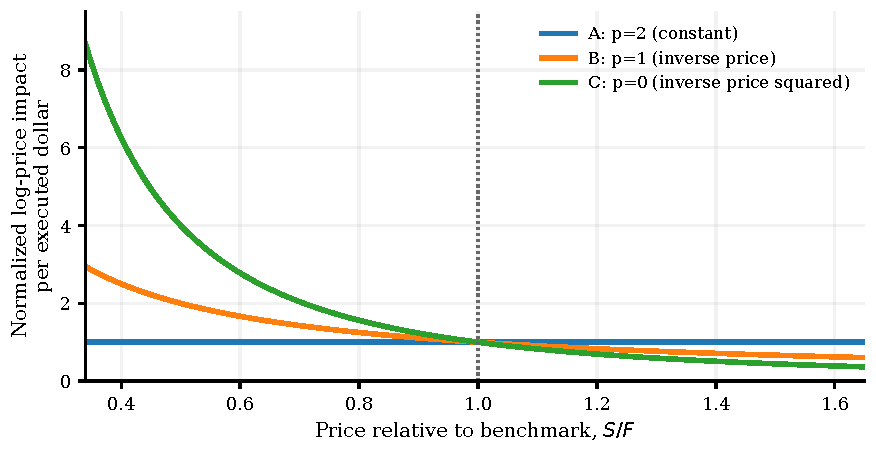
\includegraphics[width=0.82\linewidth]{figures/response_regimes.pdf}
\caption{\textbf{A single response family, three price sensitivities.} The plot shows the model-implied instantaneous \emph{log-price change per executed dollar}, normalized by its common initial value. All curves coincide at $S=F$.}\label{fig:response}
\end{figure}

Under the same executed-dollar and recovery protocol, the three response functions produce distinct attainable-state geometries. Market A supplies a global invariant-region barrier; Market B shows that nonzero partial-coverage losses need not permit arbitrarily large ones when stock inventory is finite; and Market C supplies an explicit trajectory with a severe loss. The global severity construction now extends to every fixed sublinear power-law exponent in Theorem~\ref{thm:sublinear-severe}. The condition $k<N$ in (C) is essential: at least one asset must be available to carry the compensating flow. Finite gross share rates further constrain the compensating asset's \emph{capacity}.

For $p=1$, the inventory potential from \eqref{eq:E} is
\begin{equation}\label{eq:inventoryb}
E_1(Fe^{-L})=\frac{F^2}{\eta}\left(L+e^{-L}-1\right).
\end{equation}
By \eqref{eq:cost}, terminal dollar closure and no short selling imply $E_1(S_i(T))\le FH_0$. Since $L+e^{-L}-1\to\infty$ as $L\to\infty$, no fixed finite inventory can support arbitrarily severe losses of the requisite $k$ assets. By contrast, for $p=0$, $E_0(S)=(S-F)^2/(2\eta)$ remains bounded as $S\downarrow0$; this makes the construction in (C) possible but does not by itself prove reachability.

\begin{proposition}[Local all-asset decline]\label{prop:three-pulse}
If $g$ is $C^3$ near $F$ and $e(F)<1$, then for every $N\ge2$ there exists a terminally dollar-closed, positive-price, small-amplitude three-pulse control under which \emph{every} $S_i(T)<F$. With $c=g(F)/F^2$ and $r=e^{-\rho T/2}$, the losses of a zero-sum impulse direction $\bm u$ with every $u_i\ne0$ satisfy
\begin{equation}\label{eq:three-pulse}
L_i(T)=\frac{1-e(F)}2c^2h^2u_i^2r(1-r^2)+O(h^3)>0
\end{equation}
for sufficiently small $h>0$.
\end{proposition}
\begin{proof}
Apply the executed-dollar pulses $h\bm u$, $-(1+r)h\bm u$, $rh\bm u$ at $0,T/2,T$. They are pairwise dollar-balanced and sum to zero for every asset. Taylor expansion in the coordinate $y=\Phi(S)$ gives \eqref{eq:three-pulse}; details appear in Appendix~\ref{app:local}.
\end{proof}

\begin{proposition}[Local partial-coverage decline]\label{prop:two-pulse}
Let $k<N$, $e_0=e(F)<2$, $c=g(F)/F^2$, and $r=e^{-\rho T}<2-e_0$. Select a zero-sum dollar direction with at least $k$ positive components and execute $h\bm u$ at time $0$ and $-h\bm u$ at time $T$. Then $\Cris_\alpha(T)>0$ for all sufficiently small $h>0$, and
\begin{equation}\label{eq:two-pulse}
\overline L(T)=\frac{c^2h^2}{2N}(1-r)(2-e_0-r)\sum_iu_i^2+O(h^3).
\end{equation}
\end{proposition}
\begin{proof}
The individual losses satisfy $L_i(T)=c(1-r)hu_i+O(h^2)$, while the first-order term vanishes when averaged because $\sum_i u_i=0$. The strictly positive quadratic coefficient in \eqref{eq:two-pulse} proves the result. See Appendix~\ref{app:local}.
\end{proof}

The preceding two propositions describe local reachability within this classification. A two-pulse path can generate a partial-coverage loss under a less restrictive elasticity threshold; a three-pulse path with an additional cancellation step can generate a small decline of \emph{every} asset when $e(F)<1$. The global severe-loss construction for Market C is established separately.

\paragraph{A concrete common-budget comparison} For $N=3$, $k=2$, $F=\eta=\rho=1$, $T=3$, common turnover cap $M_0=3$, and per-asset initial inventory cap $H_0=8.2$, the $p=2$ market cannot reach any positive crisis; the $p=1$ market can reach a small positive crisis but not the threshold $\delta=10$ (it would require over $9$ shares of selling by any qualifying asset); a constructive $p=0$ path reaches $\Cris_{2/3}(T)\approx13.32$ with turnover approximately $2.62$ and a maximum per-asset cumulative share sale below $3.94$. Here the large threshold $\delta=10$ serves as a theoretical stress test separating bounded from unbounded logarithmic losses. In Market C, $E_0(Fe^{-\delta})=\frac{F^2}{2\eta}(1-e^{-\delta})^2$ remains finite as $\delta\to\infty$, whereas $\log(F/S)\to\infty$ as $S\downarrow0$. Thus, while all constructed paths maintain strictly positive prices, the unbounded-loss limit probes the asymptotic $S\downarrow0$ boundary under normalized units ($F=\eta=1$). Validation code accompanies the source files.


The common trading experiment across the three response regimes is illustrated in Figure~\ref{fig:abcnum}.

\begin{figure}[tbp]
\centering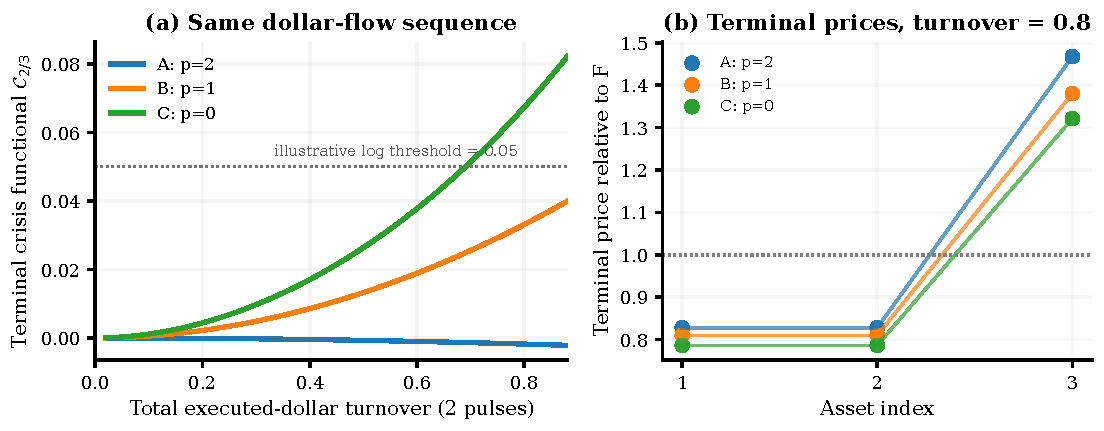
\includegraphics[width=0.98\linewidth]{figures/abc_control_comparison.pdf}
\caption{\textbf{An identical trading experiment across A/B/C response functions.} Two terminally offsetting executed-dollar pulses act on $N=3$ assets with $k=2$, $F=\eta=\rho=1$, and $T=3$. Left: the measured \emph{terminal} crisis functional as paired-dollar turnover increases; right: terminal prices under the same total turnover $M=0.8$. The dotted horizontal line marks the reference log-loss threshold 0.05.}\label{fig:abcnum}
\end{figure}

\FloatBarrier

\paragraph{The continuous power-law spectrum}
The three canonical markets in Theorem~\ref{thm:ABC} are part of a
continuous family: retain the expression for $g_p$ in
\eqref{eq:power}, now allowing $0\le p\le2$. Since $e(S)=p$,
the elasticity barriers and the local constructions distinguish
two critical exponents. In geometric terms,
$\Phi_p''(S)=(1-p)/g_p(S)$, while
$G_p''(q)=F^2(2-p)e^{(2-p)q}/\eta$ for
$G_p(q)=\Phi_p(Fe^q)$: the two curvatures reach their
respective thresholds at $p=1$ and $p=2$.
For $0\le p<2$, the dollar-coordinate
distance to zero is finite, whereas the share-coordinate distance
changes character at $p=1$:
\[
-\Phi_p(0^+)=\frac{F^2}{\eta(2-p)},\qquad
-\Psi_p(0^+)=
\begin{cases}
\displaystyle\frac{F}{\eta(1-p)},&0\le p<1,\\[3pt]
+\infty,&1\le p<2.
\end{cases}
\]
The inventory potential in~\eqref{eq:E}, evaluated at
$S=Fe^{-L}$, is for $p\ne1,2$
\[
E_p(Fe^{-L})=\frac{F^2}{\eta}
\left[\frac{e^{(p-1)L}-1}{p-1}
-\frac{1-e^{-(2-p)L}}{2-p}\right].
\]
For $0\le p<1$, its zero-price limit is
$E_p(0^+)=F^2/[\eta(1-p)(2-p)]<\infty$.
Proposition~\ref{prop:three-pulse} also makes a small, simultaneous
decline of every asset locally reachable in this regime.
Finiteness of the coordinate distances and inventory potential
alone does not establish global reachability. Theorem~\ref{thm:sublinear-severe}
below supplies the required constructive extension of uniform-budget
severe partial-coverage losses to every fixed $0\le p<1$.

At $p=1$, Theorem~\ref{thm:barrier1} excludes simultaneous declines,
while Proposition~\ref{prop:two-pulse} gives local partial-coverage
losses at every positive horizon. The potential~\eqref{eq:inventoryb}
then grows linearly with $L$. For $1<p<2$, simultaneous declines
remain excluded, but local partial-coverage losses are reachable
under the sufficient horizon condition
$e^{-\rho T}<2-p$, or $T>-\log(2-p)/\rho$.
Here the dollar distance is still finite while
$E_p(Fe^{-L})\sim F^2e^{(p-1)L}/[\eta(p-1)]$ as $L\to\infty$.
Indeed, if terminal executed-dollar flows vanish, short sales
are prohibited, and the initial inventory of a qualifying asset
is at most $H_0$,~\eqref{eq:share-bound} implies
\[
L\le\frac{1}{p-1}\log\!\left[
1+(p-1)\left(\frac{\eta H_0}{F}+\frac{1}{2-p}\right)
\right],\qquad 1<p<2.
\]
Thus, for fixed $p\in(1,2)$, the inventory-based severity
ceiling scales at most logarithmically in large $H_0$, rather than
linearly as for $p=1$. At the second threshold $p=2$,
$-\Phi_2(0^+)$ diverges and Theorem~\ref{thm:barrier2}
excludes every positive systemic crisis measure. These
thresholds distinguish local and global reachability as well
as the boundary resource singularities. Uniform severity bounds
in the sublinear regime allow constants that depend on the fixed
exponent and horizon; they do not impose a finite execution-rate cap.


\Needspace{14\baselineskip}
\begin{theorem}[Uniform-resource severe partial-coverage losses for sublinear impact]\label{thm:sublinear-severe}
Fix $N\ge2$, $k=\lceil\alpha N\rceil<N$, positive $F,\eta,\rho$,
and an exponent $0\le p<1$ in
$g_p(S)=\eta(S/F)^p$. There exist a finite horizon $T>0$
and finite constants $M_0,H_0$, depending on these fixed
market parameters but not on the loss threshold, such that for
every $\delta>0$ an admissible positive-price,
terminally dollar-closed path, using finitely many
flow-completed pulses and absolutely continuous controls
between them, satisfies
\[
\Cris_\alpha(T)>\delta,\qquad
M(\gamma)\le M_0,\qquad
H_i^-(\gamma)\le H_0\quad(1\le i\le N).
\]
No constants uniform as $p\uparrow1$ and no prescribed
finite gross execution-rate cap are asserted.
\end{theorem}
\begin{proof}
Put $\nu=2-p>1$. Paired-dollar pulses preserve
$\sum_iS_i^\nu$, so their positive-price orbits are
$\ell^\nu$ spheres. The constructive $\ell^\nu$-radial
extension of Appendix~\ref{app:severe} is given in
Appendix~\ref{app:sublinear-severe}, including per-asset
terminal dollar closure and bounds on pulse turnover,
continuous turnover, and total share sales that are
independent of the terminal target price
$\varepsilon\downarrow0$.
\end{proof}

\subsection{A sharp boundary when every asset must fall}\label{sec:allcoverage}
Market C relies on $k<N$. To see why the breadth condition matters beyond a technical assumption, keep \emph{the same constant-impact response} but change the target to $k=N$. There is then no nonqualifying asset available to compensate the other $N-1$ terminal losses. In the sharp construction, the high-price role rotates among assets during recovery; finite recovery time limits how far their common terminal price can fall. The model therefore yields an exact horizon-dependent ceiling, even before a fixed execution budget is imposed.

\begin{theorem}[Sharp all-asset horizon threshold]\label{thm:critical}
Under Assumption~\ref{asmp:model} with $g(S)=\eta$ and $k=N$, define
\begin{equation}\label{eq:critical}
\boxed{\delta_{\mathrm{crit}}(N,T)=
\log\frac{\sqrt N}{1+(\sqrt N-1)e^{-\rho T}}.}
\end{equation}
For every $\delta\in(0,\delta_{\mathrm{crit}}(N,T))$, some admissible terminally dollar-closed control reaches $\Cris_1(T)\ge\delta$ with finite turnover and sufficiently large finite inventory. If $\delta\ge\delta_{\mathrm{crit}}(N,T)$, no such positive-price path exists. Thus $\delta_{\mathrm{crit}}$ is the \emph{unattained supremum} of the all-asset common log drawdown.
\end{theorem}
\begin{proof}[Proof sketch]
Set $R(t)^2=\sum_iS_i(t)^2$. Under constant response, any paired-dollar trade satisfies $\dd R^2|_{\rm trade}=2\eta\sum_i\dd X_i=0$. Between trades,
\[
\dot R=-\rho\left(R-F\frac{\sum_iS_i}{R}\right).
\]
For positive prices, $\sum_iS_i/R>1$, whence $R(T)>F\{1+(\sqrt N-1)e^{-\rho T}\}$. If each asset ends below $Fe^{-\delta}$, then $R(T)\le F\sqrt Ne^{-\delta}$, proving necessity. For sufficiency, rotate the price vector through $N$ positive spherical directions with one high coordinate, allotting each asset equal recovery weight. Each reorientation is a zero-sum paired-dollar pulse, and paired controls during recovery keep the direction fixed. Equal terminal prices and equal recovery integrals, together with $\sum_iX_i(T)=0$, give $X_i(T)=0$ for every $i$. Moving the positive low coordinates toward zero approaches the bound continuously. A full constructive proof is in Appendix~\ref{app:sharp}.
\end{proof}


\section{Necessary execution resources}\label{sec:budget}
The response regimes determine whether a loss state is reachable. We next quantify the dollar turnover and share sales required to attain a specified breadth and severity. The following bounds apply to general positive response functions.

\begin{theorem}[Execution-resource lower bounds]\label{thm:resource}
Suppose an admissible terminal path satisfies $\Cris_\alpha(T)\ge\delta>0$. Write $k=\lceil\alpha N\rceil$ and $s=Fe^{-\delta}$. Alongside $\Phi$, define the monotone share-response coordinate $\Psi(S)=\int_F^S\dd u/g(u)$. Then the necessary dollar-turnover and total share-sale bounds are simply the respective coordinate distances to $s$:
\begin{equation}\label{eq:resource-lower}
\boxed{M\ge -k\Phi(s)=k\int_s^F\frac{u}{g(u)}\dd u,\qquad
\sum_iH_i^-\ge -k\Psi(s)=k\int_s^F\frac{\dd u}{g(u)}.}
\end{equation}
Moreover, if $X_i(T)=0$, no short sales are allowed, and the initial inventory of any qualifying asset does not exceed $H_i$, then
\begin{equation}\label{eq:share-bound}
\boxed{\int_s^F\frac{F-u}{g(u)}\dd u\le FH_i.}
\end{equation}
These necessary lower bounds need not be sharp.
\end{theorem}
\begin{proof}
For a terminally qualifying asset, the final price is at most $s<F$. Both transformed coordinates increase with price, and recovery acts toward their zero values at $F$. Consequently the cumulative negative executed-dollar and share variations must be at least $-\Phi(s)$ and $-\Psi(s)$, respectively. Summing over $k$ distinct qualifying assets proves \eqref{eq:resource-lower} because sales by qualifying assets form a subset of total sales, and each paired execution is counted once in total sales. Equation~\eqref{eq:share-bound} follows from the nonnegative right-hand side of \eqref{eq:cost} with $X_i(T)=0$ and $\theta_i(0)-\theta_i(T)\le H_i$. The detailed variation argument is given in Appendix~\ref{app:accounting}.
\end{proof}

Geometrically, the resource bounds measure distances in the two monotone coordinates. Trading direction, recovery time, and the buying capacity of receiving assets impose further requirements; we turn to these execution restrictions next.

Replicating identical asset depths at fixed $\alpha$ and $\delta$ gives $k=\Theta(N)$, and hence $M_*^{\rm end}=\Omega(N)$ for reachable targets. This experiment holds depth per asset fixed, so aggregate depth grows with $N$.

The low-price integrals discriminate different kinds of resource scarcity:
\begin{equation}\label{eq:lowprice}
\int_0^F\frac{u}{g(u)}\dd u,\qquad
\int_0^F\frac{\dd u}{g(u)}.
\end{equation}
For a local power law $g(u)\asymp u^p$, the dollar integral converges only if $p<2$, and the share integral only if $p<1$. These integral criteria separate resource feasibility from the structural and dynamic conditions for reachability.

\paragraph{Dimensionless execution scales}
Let $g_F=g(F)>0$ and define the \emph{local benchmark dollar-impact scale} $D_F=F^2/g_F$. At the benchmark, a signed executed-dollar amount $D_F$ corresponds to a unit first-order log-price displacement under the model's marginal response rule, providing an intrinsic model scale. The dimensionless controls are
\[
\widehat M=\frac{M}{D_F},\qquad
\widehat H_i=\frac{g_F H_i}{F},\qquad
\widehat v=\frac{g_F\bar v}{\rho F},\qquad
\widehat T=\rho T.
\]
For the power family $g_p(S)=\eta(S/F)^p$, the necessary dollar-turnover bound in \eqref{eq:resource-lower} becomes
\[
\widehat M\ge k\begin{cases}
\displaystyle\frac{1-e^{-(2-p)\delta}}{2-p},&p\ne2,\\[4pt]
\delta,&p=2.
\end{cases}
\]
In the ten-asset, two-session constant-impact certificate, $F=g_F=1$, $\rho=0.4$, $M<3$, $\max_iH_i^-<2$, and $\bar v_{\mathrm{used}}<0.285$ imply $\widehat M<3$, $\max_i\widehat H_i^-<2$, and $\widehat v_{\mathrm{used}}<0.7125$. Relating these dimensionless quantities to observed market depth, accessible inventory, or average daily volume requires asset-specific empirical calibration of $g_F$ and $\rho$.



\paragraph{Turnover and quadratic dissipation}
The coordinate-distance bounds of Theorem~\ref{thm:resource} can be complemented
by an aggregate estimate for constant per-share impact. Define
\[
\mathcal V_2(t)=\frac12\sum_{i=1}^N\bigl(S_i(t)^2-F^2\bigr).
\]

\begin{proposition}[Turnover--dissipation bound under constant impact]\label{prop:turnover-dissipation}
Suppose $g(S)\equiv\eta>0$ and $S_i(0)=F$. Let the paired-dollar controls
be absolutely continuous and assume that the entire price path satisfies
$S_i(t)\ge a>0$ and $|S_i(t)-F|\le b$ for all $i$ and $t\in[0,T]$.
With $\dot M(t)=\sum_e\dot z_e(t)$ and $\mathrm e=\exp(1)$, the quadratic
potential obeys the exact identity
\begin{equation}\label{eq:V2-identity}
-\mathcal V_2(T)=\frac{\rho}{2}\int_0^T
e^{-\rho(T-t)}\sum_{i=1}^N(S_i(t)-F)^2\dd t\ge0
\end{equation}
and the turnover inequality
\begin{equation}\label{eq:V2-turnover}
-\mathcal V_2(T)\le
\frac{\rho\eta b}{a}\int_0^T
(T-u)e^{-\rho(T-u)}\dot M(u)\dd u
\le\frac{\eta b}{a\,\mathrm e}M(T).
\end{equation}
\end{proposition}
\begin{proof}
Set $x_i=S_i-F$. The price equation
$\dot S_i=-\rho x_i+\eta\dot X_i/S_i$ and dollar pairing
$\sum_i\dot X_i=0$ give
\[
\dot{\mathcal V}_2
=-\rho\mathcal V_2-\frac{\rho}{2}\sum_i x_i^2,
\qquad \mathcal V_2(0)=0.
\]
Variation of constants proves~\eqref{eq:V2-identity}. Applying it to
the level-price equation and using $S_i\ge a$ yields
\[
\begin{aligned}
\sum_i|x_i(t)|
&\le\frac{\eta}{a}\int_0^t e^{-\rho(t-u)}
\sum_i|\dot X_i(u)|\dd u\\
&\le\frac{2\eta}{a}\int_0^t e^{-\rho(t-u)}
\dot M(u)\dd u.
\end{aligned}
\]
The second inequality follows from
$\sum_i|\dot X_i|\le2\sum_e\dot z_e=2\dot M$;
oppositely directed flows at an asset can cancel in the net dollar
rate. Since $\sum_i x_i^2\le b\sum_i|x_i|$, substitution into
\eqref{eq:V2-identity} and interchange of the nonnegative integrals give
the first inequality in~\eqref{eq:V2-turnover}. The second follows from
$\sup_{s\ge0}\rho s e^{-\rho s}=\mathrm e^{-1}$.
\end{proof}

The time weight $\rho(T-u)e^{-\rho(T-u)}$ in
\eqref{eq:V2-turnover} vanishes at $u=T$ and reaches its unique
maximum at $T-u=1/\rho$; it also decays for trades made far
before the terminal date. This describes the contribution of a
dollar of turnover to the \emph{upper-bound estimate}: late trades
allow little time for recovery dissipation, while earlier disturbances
decay before $T$. 

\paragraph{Two-session rolling-band example}
Consider a uniform symmetric $\pm25\%$ price band during each of two
sessions, with the second session referenced to the preceding close.
Then every price lies in
$[9F/16,25F/16]$, so $a=b=9F/16$ is admissible and
\[
-\mathcal V_2(T)\le\frac{\eta}{\mathrm e}M(T).
\]
If all $N$ assets close at or below $(1-d)F$, $0<d<1$, then
$-\mathcal V_2(T)\ge NF^2(2d-d^2)/2$, implying
\[
M(T)\ge\frac{\mathrm e\,NF^2}{2\eta}(2d-d^2).
\]
At $N=10$, $F=\eta=1$ and $d=0.02$, this becomes
$M(T)\ge0.5382$, compared with $M(T)\ge0.198$ from
Theorem~\ref{thm:resource}. Both bounds remain below $M=3$.

For partial coverage, appreciation of the compensating assets can
offset part of the falling subset's potential deficit. The aggregate
potential itself cannot become positive by~\eqref{eq:V2-identity};
without further constraints on compensating prices, it need not
provide a useful positive lower bound on turnover for a specified
falling subset alone.


\section{Finite trading rates and abstract price bands}\label{sec:rateband}
A structurally reachable loss may require trades that cannot be completed at finite speed. We therefore restrict the control set by gross executed-share rates and single-session price bands. These restrictions preserve the barrier theorems, while positive reachability requires a new continuous construction rather than the pulse controls used in Market C.

Finite-speed controls connect the execution setting to optimal trading and bounded-rate strategies \citep{AlmgrenChriss2001,Yang2019}. Here the rate limit constrains which aggregate loss states can be reached.

\subsection{Two separate execution restrictions}\label{subsec:execution-restrictions}
For absolutely continuous nonnegative paired-dollar edge rates $\dot z_e(t)$, define an asset's \emph{gross executed share rate} by
\begin{equation}\label{eq:grossrate}
 r_i^{\mathrm{gross}}(t)=\frac{1}{S_i(t)}\sum_e |B_{ie}|\dot z_e(t),\qquad
 0\le r_i^{\mathrm{gross}}(t)\le\bar v,\qquad i=1,\ldots,N.
\end{equation}
This bound counts buy and sell executions \emph{before} netting. In particular $|\dot\theta_i|\le r_i^{\mathrm{gross}}\le\bar v$ and instantaneous pulses are inadmissible. Bounding only the signed net share rate would allow simultaneous offsetting gross transactions of arbitrary size and would not constrain executed turnover.

Independently, an abstract \emph{one-session price-band constraint} restricts every executed price to
\begin{equation}\label{eq:band}
 F(1-\beta_-)\le S_i(t)\le F(1+\beta_+),\qquad
 0<\beta_-<1,\quad\beta_+>0.
\end{equation}
The control must keep the executed-price path within this interval; trajectories crossing the boundary are inadmissible. We treat \eqref{eq:band} as an abstract state constraint and defer institutional comparisons with exchange price-limit rules to Section~\ref{sec:discussion}.

\begin{proposition}[Rate and price-band exclusion certificates]\label{prop:rate-band}
Suppose the common impact function is positive and $g(S)\le G$ on the whole admissible price region. Under the cap~\eqref{eq:grossrate}, every asset obeys
\begin{equation}\label{eq:rate-floor}
 S_i(t)\ge F-\frac{G\bar v}{\rho}(1-e^{-\rho t}),\qquad 0\le t\le T.
\end{equation}
Under the additional price band~\eqref{eq:band}, put
\begin{equation}\label{eq:twofloors}
 S_{\rm floor}=\max\!\left\{F(1-\beta_-),\;F-\frac{G\bar v}{\rho}(1-e^{-\rho T})\right\}>0.
\end{equation}
Then for any breadth $\alpha$ and any admissible control,
\begin{equation}\label{eq:constrained-crisis}
\boxed{\ \mathcal C_\alpha(t)\le \log\frac{F}{S_{\rm floor}}\quad\hbox{for all }t\le T.\ }
\end{equation}
In particular, a necessary finite-speed condition to reach threshold $\delta>0$ is
\begin{equation}\label{eq:min-speed}
\boxed{\ \bar v\ge\frac{\rho F(1-e^{-\delta})}{G(1-e^{-\rho T})}.\ }
\end{equation}
A one-session lower price limit independently excludes any $\delta> -\log(1-\beta_-)$. These are \emph{necessary} constraints, generally not sharp reachability thresholds. For comparison, if a \emph{hypothetical} multi-session regime resets a proportional lower band to each preceding close, then over $D$ sessions the elementary bound is only
$S_i(T_D)\ge F\prod_{d=1}^D(1-\beta_{-,d})$ and
$\mathcal C_\alpha(T_D)\le-\sum_{d=1}^D\log(1-\beta_{-,d})$.
The cumulative ceiling depends on the successive closing-price resets.
\end{proposition}
\begin{proof}
The variation-of-constants formula for $\dot S_i=-\rho(S_i-F)+g(S_i)\dot\theta_i$ and $|\dot\theta_i|\le\bar v$ yields $S_i(t)\ge F-G\bar v\int_0^t e^{-\rho(t-s)}\dd s$, proving \eqref{eq:rate-floor}. The price band supplies the second floor; every individual log loss is at most $\log(F/S_{\rm floor})$, and so are its cross-sectional mean, upper-breadth threshold, and their minimum. Rearranging the rate-only floor is necessary for an individual loss to reach $\delta$.
\end{proof}

Dollar pairing and terminal closure yield additional market-wide execution requirements. Since each paired dollar is counted twice in gross share execution,
\begin{equation}\label{eq:rate-turnover}
 M=\frac12\int_0^T\sum_i S_i(t)r_i^{\mathrm{gross}}(t)\dd t
 \le\frac{NF(1+\beta_+)\bar v T}{2}.
\end{equation}
Together with Theorem~\ref{thm:resource}, this gives the necessary joint constraint
\begin{equation}\label{eq:rate-budget-lower}
 \boxed{\ \bar v\ge\frac{2k}{NF(1+\beta_+)T}
 \int_{Fe^{-\delta}}^F\frac{u}{g(u)}\dd u.\ }
\end{equation}
For a closed executed-dollar ledger, the nonnegative cost identity~\eqref{eq:cost} also yields
\begin{equation}\label{eq:rate-energy}
 E(S_i(T))\le F\bar v T,\qquad
 \bar v\ge \frac{E(Fe^{-\delta})}{FT}
 \quad \hbox{for every qualifying asset.}
\end{equation}
Bounds~\eqref{eq:min-speed}, \eqref{eq:rate-budget-lower}, and \eqref{eq:rate-energy} impose complementary restrictions on execution rates.

A per-asset rate estimate gives a first-order $O(\bar v)$ bound on systemic losses. Under dollar pairing, the leading-order price movements cancel in the market mean, yielding the quadratic small-rate bound below for constant impact.

\begin{theorem}[A quadratic small-rate crisis barrier for constant impact]\label{thm:quadratic-rate}
Let $g(S)\equiv\eta>0$, assume dollar pairing $\sum_iS_i\dot\theta_i=0$, and impose the gross share-rate cap~\eqref{eq:grossrate}. Write $d_T=1-e^{-\rho T}$ and
\begin{equation}\label{eq:bsmall}
 b_T=\frac{\eta\bar v}{F\rho}\,d_T<1.
\end{equation}
Then, with or without terminal dollar closure and for \emph{every} $N\ge2$ and breadth $\alpha$,
\begin{equation}\label{eq:quadratic-rate}
\boxed{\ \mathcal C_\alpha(T)\le
\left(\frac{\eta\bar v}{F\rho}\right)^2
\left[d_T-\rho T e^{-\rho T}
 +\frac{d_T^2}{2(1-b_T)^2}\right].\ }
\end{equation}
Consequently, the supremum of attainable systemic losses is $O(\bar v^2)$ as $\bar v\downarrow0$. For fixed $N,T$ and positive price-band widths on both sides of the benchmark, Theorem~\ref{thm:finite-rate-construct} supplies a matching construction. Here $\bar v_*(\delta)$ denotes the infimum rate cap permitting severity at least $\delta$, with fixed $N,T,F,\rho,\eta,\alpha$, positive per-asset initial inventory allowances, terminal dollar closure, and prescribed bands $\beta_->0$, $\beta_+>0$. In this constrained class, $\bar v_*(\delta)=\Theta(\sqrt\delta)$ as $\delta\downarrow0$. These bounds determine the scaling order; the optimal constants remain undetermined.
\end{theorem}
\begin{proof}
Set $x_i(t)=S_i(t)-F$ and $m(t)=\sum_i x_i(t)$. Variation of constants gives
$|x_i(t)|\le\eta\bar v(1-e^{-\rho t})/\rho$. Since $\sum_iS_i\dot\theta_i=0$,
$\sum_i\dot\theta_i=-F^{-1}\sum_i x_i\dot\theta_i$ and therefore
$\dot m=-\rho m-(\eta/F)\sum_i x_i\dot\theta_i$. Integrating and bounding the gross rates yields
\begin{equation}\label{eq:meanprice}
\frac{|m(T)|}{NF}\le
\left(\frac{\eta\bar v}{F\rho}\right)^2
 [d_T-\rho T e^{-\rho T}].
\end{equation}
For $|x_i(T)|/F\le b_T<1$, Taylor's inequality
$-\log(1+y)\le-y+y^2/[2(1-b_T)^2]$ implies
$\overline L(T)\le |m(T)|/(NF)+b_T^2/[2(1-b_T)^2]$.
Use $\mathcal C_\alpha\le\overline L$ to obtain~\eqref{eq:quadratic-rate}. The construction in Theorem~\ref{thm:finite-rate-construct} has $\mathcal C_1(T)=c_Na^2+O(a^3)$ with $c_N>0$, and its gross rate is $O(a)$; setting $a\propto\bar v$ gives a positive loss of matching order $\Omega(\bar v^2)$ while keeping a fixed positive band. This proves the stated small-rate exponent.
\end{proof}

\begin{theorem}[Positive all-asset decline with bounded continuous execution]\label{thm:finite-rate-construct}
Assume $g\in C^3$ near $F$, $g(F)>0$, $\rho>0$, and $e_0=Fg'(F)/g(F)<1$. Fix \emph{any} $N\ge2$, horizon $T>0$, rate cap $\bar v>0$, one-session band widths $\beta_-,\beta_+>0$, and any fixed positive amount of initially available shares per asset. Then there exists an \emph{absolutely continuous}, paired-dollar, per-asset gross-rate-bounded control, remaining strictly inside the band, with $X_i(T)=0$ for each asset and
\begin{equation}\label{eq:local-speed-crash}
 \boxed{\ S_i(T)<F\ \text{for every }i,\qquad \mathcal C_1(T)>0.\ }
\end{equation}
The attained loss can be arbitrarily small. This does \emph{not} assert that a prescribed fixed large threshold remains reachable under an arbitrarily tight cap or band.
\end{theorem}
\begin{proof}
Choose a zero-sum vector $u\in\R^N$ with every $u_i\ne0$. Put $\Delta=T/3$, $r=e^{-\rho\Delta}$ and set the bounded, three-bin signal
\begin{equation}\label{eq:bounded-control}
 f(t)=
 \begin{cases}
 1,&0\le t<\Delta,\\
 -(1+r),&\Delta\le t<2\Delta,\\
 r,&2\Delta\le t\le T,
 \end{cases}
 \qquad \dot X_i=a u_i f(t).
\end{equation}
The dollar rates sum to zero, and $\int_0^T f(t)\dd t=0$.
\par
Direct integration also gives $\int_0^T e^{-\rho(T-t)}f(t)\dd t=0$.
Write $h(S)=g(S)/S$ and expand
$S_i(t)=F+a u_i y(t)+a^2u_i^2 z(t)+O(a^3)$,
where $\dot y=-\rho y+h(F)f$, $y(0)=0$, and
$\dot z=-\rho z+h'(F)f y$, $z(0)=0$.
The weighted cancellation implies $y(T)=0$. Since $h'(F)/h(F)=(e_0-1)/F$, integration by parts yields
\begin{equation}\label{eq:finite-rate-coefficient}
 \boxed{\ \log\frac{F}{S_i(T)}=
 \frac{\rho(1-e_0)}{2F^2}\,a^2u_i^2
 \int_0^T e^{-\rho(T-t)}y(t)^2\dd t+O(a^3).\ }
\end{equation}
The integral is strictly positive. Thus all prices fall for every sufficiently small $a>0$. Represent each zero-sum dollar-rate vector by nonnegative source-to-destination edge rates with minimum gross flow, so $r_i^{\mathrm{gross}}=|a u_i f|/S_i$. The entire price path converges uniformly to $F$ as $a\downarrow0$, ensuring compliance with the rate cap, price band, and any positive inventory allowance for sufficiently small $a$.
\end{proof}

The continuous construction establishes local common-loss reachability under a finite rate cap and terminal dollar closure.

\paragraph{Interaction of rate and price-band constraints}
The global barrier for $e(S)\ge2$ and the full-coverage exclusion for $e(S)\ge1$ remain valid after restricting the set of admissible controls. For $p=1$, a bounded two-stage buy-then-sell dollar-rate control still makes $k<N$ assets end below $F$: its per-asset signed dollars integrate to zero, while $\sum_i S_i(T)=NF$ and strict concavity of $\log$ makes the average log loss positive. In contrast, the \emph{arbitrarily severe} construction for $p=0$ in Theorem~\ref{thm:ABC}(C) uses instantaneous sweeps and therefore falls outside the rate-constrained class~\eqref{eq:grossrate}. Under a fixed price band, no one-session terminal loss can exceed $-\log(1-\beta_-)$. Theorem~\ref{thm:finite-rate-construct} establishes strictly positive local all-asset declines under both restrictions, with severity limited by the rate and price-band constraints.

\begin{table}[H]\centering\small
\caption{How execution restrictions affect reachability for $p=0$. Arbitrarily severe partial-coverage losses use a sufficiently long fixed finite horizon, as in Theorem~\ref{thm:ABC}(C). Local reachability holds for every $T>0$; ``local'' refers to a sufficiently small positive terminal all-asset loss.}
\label{tab:regulatory}
\begin{tabularx}{\linewidth}{@{}>{\raggedright\arraybackslash}p{0.20\linewidth}>{\raggedright\arraybackslash}X>{\raggedright\arraybackslash}X@{}}\toprule
Admissible controls & Established reachability & Scope of the result \\ \midrule
Instantaneous sweeps, no band & Arbitrarily severe partial-coverage log loss, $k<N$ & Does not model a bounded execution rate \\
Gross rate $\bar v$ only & Local all-asset loss for any $\bar v>0$ & Unbounded severe-loss construction not certified \\
Hard session band only & Local all-asset loss when $\beta_->0$ and $\beta_+>0$ & $\delta>-\log(1-\beta_-)$ impossible \\
Both restrictions & Local all-asset loss for positive caps/widths; rate and price-floor certificates & No general exact severe threshold or optimal execution rate \\ \bottomrule
\end{tabularx}
\end{table}


Figure~\ref{fig:localrate} compares the numerical small-rate loss with its leading-order quadratic prediction.

\begin{figure}[tbp]\centering
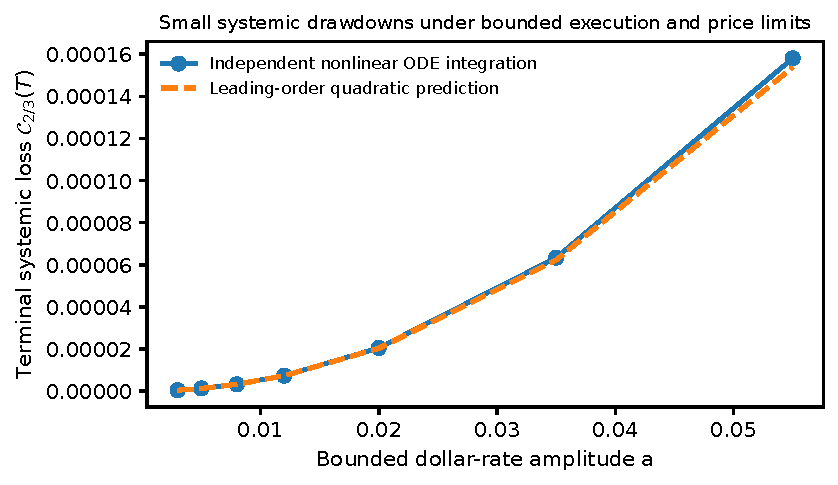
\includegraphics[width=0.76\linewidth]{figures/finite_rate_quadratic.pdf}
\caption{\textbf{Quadratic local all-asset loss under a finite-rate control.} Independently integrated nonlinear price paths for constant $g$ agree with the leading-order quadratic prediction from~\eqref{eq:finite-rate-coefficient} as the amplitude decreases. The displayed functional is $\Cris_{2/3}(T)$, evaluated for the all-asset-decline construction of Theorem~\ref{thm:finite-rate-construct}. The plotted amplitude is sufficiently small to preserve positive prices; the admissibility checks for the highlighted $a=0.035$ case are reported in the code bundle.}\label{fig:localrate}
\end{figure}


\FloatBarrier
\section{Systemic drawdowns under rolling price-band constraints}\label{sec:multiday}
We now extend the reachability analysis to a multi-session proportional-reset price-band protocol. In each session, permitted execution prices are referenced to the preceding close. Trading interruptions can shift orders forward in time and redirect pressure across markets, as the circuit-breaker analysis of Subrahmanyam~\citep{Subrahmanyam1994} illustrates. Here repeated lower-band closes couple the crisis functional to the capacity of the remaining assets to absorb paired-dollar flow. Feasibility depends jointly on breadth, mean loss, selling speed, and receiving capacity within the prescribed rate caps and bands.

Throughout, a \emph{lower-band close} (also called a \emph{lower-limit close} in some theorem statements) means that the terminal executed price attains the modeled session floor. Institutional features such as resting order queues or trading halts lie outside the executed-price state space (see Section~\ref{sec:discussion}).

\subsection{Rolling bands and the exact cumulative accounting}\label{subsec:multiday-protocol}
Partition trading time into $D$ sessions $[T_{d-1},T_d]$, each of duration $\tau_d>0$. Overnight calendar time does not contribute to the model clock; prices carry over continuously from the preceding close. In the stylized \emph{proportional-reset} version, set $R_{i,d}=S_i(T_{d-1})$ and require
\begin{equation}\label{eq:rolling-band}
 (1-\beta_{i,d,-})R_{i,d}\le S_i(t)\le(1+\beta_{i,d,+})R_{i,d},
 \qquad t\in[T_{d-1},T_d],
\end{equation}
where $0<\beta_{i,d,-}<1$. A lower-limit close is
$S_i(T_d)=(1-\beta_{i,d,-})R_{i,d}$; a $D$-day streak means this equality holds for the \emph{same} assets in $D$ consecutive sessions. A streak in $k=\lceil\alpha N\rceil$ assets is not yet a systemic crisis under Definition~\ref{def:crash}: the market-average log loss must also reach the chosen threshold.

For a common constant lower fraction $q=1-\beta_-$, each streaking asset has
$S_i(T_D)=Fq^D$ and loss $L_i(T_D)=D\lambda$ with $\lambda=-\log q$. Conversely, even without a streak, the state constraint ensures
\begin{equation}\label{eq:rolling-cumulative-upper}
  \Cris_\alpha(T_D)\le D\lambda
\end{equation}
for a common band and initial equal benchmark price. For heterogeneous bands the right side can be replaced by
$\max_i\sum_{d=1}^D[-\log(1-\beta_{i,d,-})]$. These geometric ceilings precede the execution constraints examined below.


\subsection{Cross-sectional crisis threshold under repeated lower-band closes}\label{subsec:multiday-breadth}
Consecutive lower-limit closes by $k$ stocks satisfy the breadth requirement, but do not automatically satisfy the mean-loss requirement: the remaining assets may appreciate as they receive matched dollars. This is the same $k<N$ compensation mechanism that permits Market C's partial-coverage outcomes, now seen from the opposite direction. The following exact endpoint identity shows when the falling majority becomes a crisis under the \emph{unchanged} functional, without yet constructing the trades.
\begin{proposition}[A conditional systemic-crisis trigger test]\label{prop:multiday-crisis-trigger}
Suppose the same $k=\lceil\alpha N\rceil<N$ assets close at $Fq^D$ after $D$ identical proportional-reset sessions, with $q\in(0,1)$. Let the remaining $N-k$ assets close at $Y_j>0$, and write $\lambda=-\log q$. For any $0<\delta\le D\lambda$, the \emph{terminal} crisis threshold $\Cris_\alpha(T_D)\ge\delta$ holds if and only if
\begin{equation}\label{eq:multiday-trigger-product}
\boxed{\qquad \prod_{j=1}^{N-k}\frac{Y_j}{F}
 \le\exp\bigl(kD\lambda-N\delta\bigr).\qquad}
\end{equation}
If all other assets have individual log losses at most $D\lambda$ (or if $k>N/2$, so the $N-k$ other assets cannot fill the top $k$ ranks), then $Q_\alpha(T_D)=D\lambda$ and the terminal crisis severity is exactly
\begin{equation}\label{eq:multiday-trigger-exact}
\boxed{\quad\Cris_\alpha(T_D)=\min\!\left\{D\lambda,
 \frac{kD\lambda-\sum_{j=1}^{N-k}\log(Y_j/F)}{N}\right\}.\quad}
\end{equation}
In particular, with a single compensator ($k=N-1$), its terminal price must obey $Y/F\le\exp(kD\lambda-N\delta)$ if a crisis of threshold $\delta$ is to occur. These are exact \emph{conditional endpoint identities}, not sufficient conditions for a trade path realizing the stipulated closing prices.
\end{proposition}
\begin{proof}
The $k$ streaking assets have loss $D\lambda$, hence $Q_\alpha\ge D\lambda$. For $\delta\le D\lambda$, the coverage part of the crisis criterion is therefore automatic, and the remaining requirement is $\overline L(T_D)\ge\delta$. Substituting the terminal prices into $\overline L(T_D)=N^{-1}\sum_i\log[F/S_i(T_D)]$ gives \eqref{eq:multiday-trigger-product}. If every other loss is at most $D\lambda$, or if $N-k<k$, the $k$th-largest loss is exactly $D\lambda$, proving \eqref{eq:multiday-trigger-exact}.
\end{proof}
For the interval-certified $N=10$, $k=9$, $q=0.97$, $D=2$ construction of Proposition~\ref{prop:certified-v7}, $D\lambda\approx0.060918$. The compensator closes at $Y/F\approx1.405161$ in the high-accuracy reconstruction, yielding $\Cris_{0.9}\approx0.020811$. The outward-rounded certificate gives $1.4047874<Y/F<1.4055543$, which rigorously implies $\Cris_{0.9}>0.020$ for the specified trajectory. The threshold $\delta=0.020$ requires $Y/F\le\exp(9D\lambda-10(0.020))\approx1.416609$, which the certified path satisfies. Thus the receiving asset's terminal price determines whether the same broad lower-limit streak qualifies as a systemic loss event.

Figure~\ref{fig:multiday-crisis-trigger} illustrates the distinction between repeated closing-limit losses and the systemic crisis criterion.

\begin{figure}[tbp]\centering
 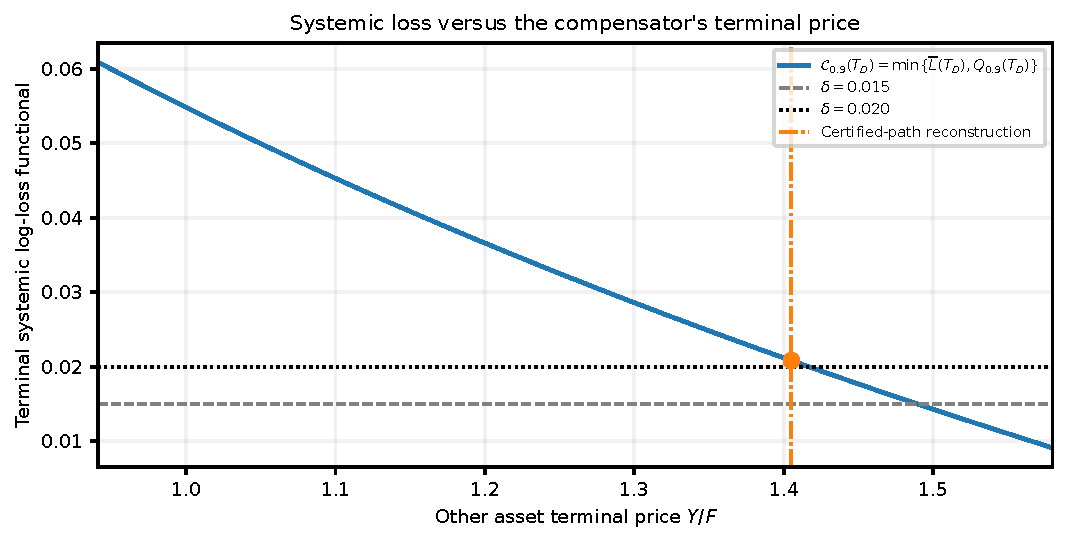
\includegraphics[width=0.85\linewidth]{figures/multiday_crisis_trigger.pdf}
 \caption{\textbf{Systemic loss and the compensating asset's terminal price.} Conditional terminal severity for $N=10$, nine assets closing twice at a 3\% daily lower limit, versus the remaining asset's terminal price. The dotted marker denotes the constructed dollar-closed path; the reference lines show the log-loss thresholds $\delta=0.015$ and $\delta=0.020$. The curve gives the conditional algebraic relation between the terminal price and systemic loss.}\label{fig:multiday-crisis-trigger}
\end{figure}

\subsection{A minimum speed for consecutive lower-band closes}\label{subsec:multiday-rate}
A closing price at the lower limit must be reached in finite time despite recovery toward $F$. For $g(S)\equiv\eta$, start a session at price $s$ and suppose its length is $\tau$ and its lower floor is $(1-\beta)s$. Even before asking who purchases the matched dollars, the gross share-rate cap bounds the fastest decline through $\dot z=-\rho(z-F)-\eta\bar v$, $z(0)=s$. This yields a necessary threshold but leaves the market-wide matching problem unresolved.
\begin{proposition}[Rolling-limit shock-rate certificates]\label{prop:rolling-rate}
In the constant per-share impact model, a lower-limit close in a session starting at $s>0$ requires
\begin{equation}\label{eq:single-session-streak-rate}
 \boxed{\quad\bar v\ge \left[\frac{\rho}{\eta}\left(F-s+
 \frac{\beta s}{1-e^{-\rho\tau}}\right)\right]_+.\quad}
\end{equation}
If the same asset closes at the same proportional lower limit on each of $D$ sessions of common duration $\tau$, with $s_d=Fq^{d-1}$, then
\begin{equation}\label{eq:D-streak-speed}
\boxed{\quad\bar v\ge\frac{\rho F}{\eta}\max_{1\le d\le D}
 \left[1+q^{d-1}\left(\frac{1-q}{1-e^{-\rho\tau}}-1\right)\right].\quad}
\end{equation}
Moreover, when $\eta\bar v<\rho F$, all prices starting at $F$ obey the perpetual \emph{rate-only} floor $S_i(t)\ge F-\eta\bar v/\rho$, implying the necessary integer-streak bound
\begin{equation}\label{eq:streak-D-bound}
\boxed{\quad D\le\frac{\log(1-\eta\bar v/(\rho F))}{\log q}.\quad}
\end{equation}
The bound is understood only for $\eta\bar v<\rho F$; with a larger rate cap it supplies no finite-day obstruction. None of these scalar inequalities is sufficient for multi-asset price-band feasibility or terminal dollar closure.
\end{proposition}
\begin{proof}
Variation of constants and $\dot\theta_i\ge-\bar v$ imply
$S_i(\tau)\ge F+(s-F)e^{-\rho\tau}-(\eta\bar v/\rho)(1-e^{-\rho\tau})$.
Requiring $S_i(\tau)\le(1-\beta)s$ yields \eqref{eq:single-session-streak-rate}; substitute $s=Fq^{d-1}$ for each day to obtain \eqref{eq:D-streak-speed}. The same scalar comparison from initial $F$ gives $S_i(t)\ge F-(\eta\bar v/\rho)(1-e^{-\rho t})$, hence the uniform floor; combine it with $Fq^D$ and note $\log q<0$ to deduce \eqref{eq:streak-D-bound}.
\end{proof}


\subsection{Obstruction to universal consecutive lower-band closes}\label{subsec:multiday-full}
The all-asset case is especially restrictive: there is no complement capable of absorbing a net dollar flow. The same potential that gave the original exclusion barriers now rules out a second simultaneous decline under a simple below-benchmark band condition. This obstruction extends the breadth distinction in the A/B/C regimes to the entire market.
\begin{theorem}[An obstruction to a second all-asset limit-down close]\label{thm:no-second-global}
Assume $g_i(S)>0$, $\rho_i>0$, unchanged fundamental benchmarks $F_i>0$, and instantaneous interasset executed-dollar balance $\sum_i\dd X_i=0$. Suppose every asset closes the first session at $S_i(T_1)=q_iF_i<F_i$, and the \emph{entire second-session admissible band} lies at or below its own benchmark,
\begin{equation}\label{eq:no-second-condition}
 (1+\beta_{i,2,+})q_i\le1\quad\text{for every }i.
\end{equation}
Then it is impossible for \emph{every} asset to close the second session strictly below its first close. In particular, simultaneous second-day lower-limit closes in all $N$ assets are impossible. This holds regardless of the transaction-rate cap, terminal signed-dollar balances, or the functional form of the positive $g_i$.
\end{theorem}
\begin{proof}
Use $\Phi_i'(S)=S/g_i(S)>0$ and $H=\sum_i\Phi_i(S_i)$. Trade settlement preserves $H$, and recovery contributes
$\dot H=-\sum_i\rho_i S_i(S_i-F_i)/g_i(S_i)\ge0$ whenever every $S_i\le F_i$.
Condition~\eqref{eq:no-second-condition} keeps the full second-session price path in that region. Hence $H(T_2)\ge H(T_1)$. If every second close were below the preceding close, strict monotonicity of all $\Phi_i$ would instead give $H(T_2)<H(T_1)$, a contradiction.
\end{proof}

For the stylized symmetric proportional band, $q_i=1-\beta_i$ and
$\beta_{i,2,+}=\beta_i>0$, so
$(1+\beta_i)(1-\beta_i)=1-\beta_i^2<1$ and the theorem applies. The theorem uses full execution, paired-dollar settlement, and fixed fundamentals. Extensions with unmatched orders, an external cash account, or changing fundamentals require separate analysis. It leaves open consecutive streaks in $k<N$ assets supported by offsetting dollar flows in the remaining assets.


The same model cannot represent a positive-duration \emph{all-asset locked limit-down state} with every price fixed strictly below $F_i$: maintaining $\dot S_i=0$ would require
$\dot X_i=\rho_i S_i(S_i-F_i)/g_i(S_i)<0$ for every asset, contradicting $\sum_i\dot X_i=0$. A limit-hit closing print is instead permitted as an endpoint condition. Persistent unmatched sell queues require a new order-book state, not simply an extended price trajectory.

\subsection{A positive multi-day resource and accounting constraint}\label{subsec:multiday-preconditioning}
Even when not all assets fall, each target that is below $F$ faces upward recovery. Terminal dollar closure therefore requires a path-history resource, not just a final selling flow: earlier above-benchmark excursions must provide the positive recovery contribution that compensates later losses. This is another expression of the same potential introduced in Section~\ref{sec:barriers}, now integrated over successive trading sessions.
\begin{proposition}[Preconditioning needed for a dollar-closed limit-down streak]\label{prop:streak-precondition}
Let an asset begin at $F$ and finish $D$ sessions at $s_D<F$, with $X_i(T_D)=0$. Then its trajectory necessarily visits $S_i>F$ on a set of positive trading-time measure and satisfies
\begin{equation}\label{eq:streak-excursion}
 \rho\int_0^{T_D}\frac{S_i(t)(S_i(t)-F)}{g(S_i(t))}\dd t
 =\int_{s_D}^{F}\frac{u}{g(u)}\dd u>0.
\end{equation}
If every session after the first keeps the asset at or below $F$, and the first-session upper band is $U_1>F$, a necessary condition is
\begin{equation}\label{eq:streak-precondition}
 \boxed{\quad \rho\tau_1\max_{F\le u\le U_1}\frac{u(u-F)}{g(u)}
 \ge \int_{s_D}^{F}\frac{u}{g(u)}\dd u.\quad}
\end{equation}
For constant impact $g=\eta$, and $s_D=Fq^D$, $U_1=F(1+\beta_+)$, this simplifies to
$\rho\tau_1\ge(1-q^{2D})/[2\beta_+(1+\beta_+)]$.
Writing $H_+=\rho\tau_1\beta_+(1+\beta_+)$, whenever $2H_+<1$ this imposes the additional necessary streak-length bound
\begin{equation}\label{eq:multiday-preconditioning-D}
\boxed{\quad D\le \frac{\log(1-2H_+)}{2\log q}.\quad}
\end{equation}
This bound is specific to terminal dollar closure and the absence of above-fundamental excursions in later sessions. It is not sufficient to produce a consecutive limit-down path.
\end{proposition}
\begin{proof}
Integrate the identity $\dd\Phi(S_i)=\dd X_i-\rho S_i(S_i-F)\dd t/g(S_i)$ over the full horizon. Since $X_i(T_D)=0$ and $\Phi(F)=0$, the integral must equal $-\Phi(s_D)>0$. Any portion of the trajectory at $S_i\le F$ contributes a nonpositive integrand, so the positive part must arise above $F$. If later sessions cannot rise above $F$, all positive contribution must be earned in session~1, whose supremum is bounded by the left side of \eqref{eq:streak-precondition}.
\end{proof}


\subsection{A necessary receiving-capacity bound for multiasset execution}\label{subsec:multiday-cut}
For $k<N$, a subset's net executed-dollar outflow must be absorbed by the remaining assets. Partition the assets into a falling subset $J$ and its complement $J^c$. On a complete trading graph with node-level gross-rate caps and no separate edge capacities, conservation and the receiving assets' prices and rates bound the dollar flow across this partition.
\begin{proposition}[A market-cut capacity and consecutive-limit lower bound]\label{prop:market-cut}
Fix a subset $J$ of assets and write $J^c$ for its complement. Under paired-dollar execution and the per-asset gross share-rate cap $\bar v$, every admissible absolutely continuous path satisfies, for almost every $t$,
\begin{equation}\label{eq:market-cut-instant}
\boxed{\left|\sum_{i\in J}\dot X_i(t)\right|\le
\bar v\min\left\{\sum_{i\in J} S_i(t),\sum_{j\in J^c}S_j(t)\right\}.}
\end{equation}
Suppose that throughout a session $[T_{d-1},T_d]$ of length $\tau_d$, each $i\in J$ stays at or below its unchanged benchmark $F_i$ and ends at $s_{i,d}<s_{i,d-1}$. Let $\Phi_i'(S)=S/g_i(S)>0$ and put
\begin{equation}\label{eq:cut-required}
K_{J,d}:=\sum_{i\in J}\big[\Phi_i(s_{i,d-1})-\Phi_i(s_{i,d})\big]>0.
\end{equation}
If all compensating assets satisfy $S_j(t)\le U_{j,d}$ during that session, then the session's paired executed-dollar turnover $M_d$ and the required gross-share-rate cap satisfy
\begin{equation}\label{eq:cut-necessary}
\boxed{M_d\ge K_{J,d},\qquad
\bar v\ge\frac{K_{J,d}}{\tau_d\sum_{j\in J^c}U_{j,d}}.}
\end{equation}
When $J^c=\varnothing$, the hypothesized simultaneous strict decrease of all assets cannot occur on a session lying entirely below benchmarks.
\end{proposition}
\begin{proof}
Dollar pairing gives $\sum_{i\in J}\dot X_i=-\sum_{j\in J^c}\dot X_j$. In either set, $|\dot X_i|\le S_i r_i^{\mathrm{gross}}\le S_i\bar v$, proving~\eqref{eq:market-cut-instant}. The price-response coordinate obeys
$\Delta X_i=\Phi_i(s_{i,d})-\Phi_i(s_{i,d-1})+
\rho_i\int_{T_{d-1}}^{T_d}S_i(S_i-F_i)/g_i(S_i)\dd t$.
The integral is nonpositive for $i\in J$, hence $\sum_{i\in J}\Delta X_i\le-K_{J,d}$. The net executed dollars entering $J^c$ are therefore at least $K_{J,d}$. The total matched-dollar turnover must cover this flow, and the complement's gross-share capacity is no more than $\bar v\tau_d\sum_{j\in J^c}U_{j,d}$. These yield~\eqref{eq:cut-necessary}. If $J^c$ is empty, there is no opposing flow.
\end{proof}
A nonempty complement can impose an additional rate requirement through its receiving capacity. Its appreciation also offsets the market-average log loss in Proposition~\ref{prop:multiday-crisis-trigger}, so feasibility depends on both dollar absorption and the resulting average loss.

For constant per-share impact $g_i\equiv\eta$, $k=|J|$ identical lower-limit assets, initial benchmark $F$, common lower-limit ratio $q\in(0,1)$, and $m=N-k$ compensators with common upper-band fraction $\beta_{c,+}$, the $d$th-day specialization is
\begin{equation}\label{eq:cut-special}
\boxed{\bar v\ge \frac{k}{m}\,
\frac{F\,\big(q^{2(d-1)}-q^{2d}\big)}{2\eta\tau_d(1+\beta_{c,+})^{d}}\quad(d\ge2),}
\end{equation}
provided all $k$ target prices remain below $F$ and each compensator's preceding reference price has evolved from $F$ under the specified upper bands. The $k/m$ multiplier makes the funding bottleneck explicit. The condition gives a \emph{necessary} lower bound on the rate. For the ten-asset, two-day example ($k=9,m=1,q=0.97,\beta_{c,+}=0.25,\tau_d=20$), it gives only $\bar v\gtrsim 0.0080$; the stronger systemic quadratic bound below is more informative for that particular configuration.

\subsection{A certified two-session construction and bounds on the critical rate}\label{subsec:v7-certified}
We construct and certify a path satisfying all the preceding constraints. Fix $N=10$, with nine identical target assets and one compensator, $F=\eta=1$, $\rho=0.4$, two sessions of length $20$, target rolling bands $\pm3\%$, compensator bands $\pm25\%$, and terminal closure $X_i(40)=0$ for every asset. The targets share one prescribed continuous price path $x(t)$; the compensator follows the scalar nonlinear ODE determined by paired dollars. This symmetry reduces the calculation to two price states and establishes feasibility for the specified ten-asset model. A reproducible fixed-point interval calculation certifies the nonlinear compensator dynamics and all execution constraints for the piecewise-linear target path.
\begin{proposition}[A computer-assisted two-day rate certificate]\label{prop:certified-v7}
In the ten-asset specification above ($k=9$, $F=\eta=1$, $\rho=0.4$, $\tau_1=\tau_2=20$, target bands $\pm3\%$, compensator bands $\pm25\%$), there exists an absolutely continuous, fully paired-dollar path with all per-asset terminal signed-dollar ledgers exactly zero such that the same nine assets close at $0.97$ and $0.9409$, respectively, while
\begin{equation}\label{eq:v7-certified-result}
\boxed{\Cris_{0.9}(40)>0.020,\quad \bar v_{\mathrm{used}}<0.285,\quad M<3,\quad H_i^-<2\quad(1\le i\le10).}
\end{equation}
Every executed price remains inside its rolling session band. Here $M$ counts paired executed dollars once and $H_i^-$ denotes gross shares sold, so initial holdings of two shares of every asset are sufficient without shorting.
\end{proposition}
\begin{proof}[Proof sketch]
Let $r=23/10$. Prescribe the common target price $x(t)$ as the continuous piecewise-linear interpolation of
\begin{equation}\label{eq:v7-knots}
(t,x)=(0,1),(r,h),(20-r,h),(20,0.97),(20+r,0.995),(40-r,0.995),(40,0.9409).
\end{equation}
The first plateau $h$ is the unique root near $1.02$ of the exact net-dollar-closure equation
\begin{equation}\label{eq:v7-root}
\begin{aligned}
&101600000000h^2-97138000000h-6646157699=0,\\
&1.02020225507905<h<1.02020225507908.
\end{aligned}
\end{equation}
The compensator $y(t)$ is the unique positive solution of
$\dot y=-0.4(y-1)-9u(t)/y$, $y(0)=1$, where
$u(t)=x(t)[\dot x(t)+0.4(x(t)-1)]$.
All ten executed-dollar flows sum to zero at each time, and the exact root equation gives $X_i(40)=0$ for every target, hence also for the compensator. A validated interval integration gives
\begin{equation}\label{eq:v7-bounds}
\begin{gathered}
1.2219388<y(20)<1.2225356,\quad
1.4047874<y(40)<1.4055543,\\
\sup_t9|u(t)|/y(t)<0.284481,\\
\int_0^{40}9[u(t)]_+/y(t)\dd t<1.880,\qquad
9\int_0^{40}|u(t)|\dd t<2.984.
\end{gathered}
\end{equation}
The targets have even smaller gross rates and gross selling shares; sessionwise interval enclosures verify both rolling bands. Exact rational enclosures for $e^{0.2}$ verify $\overline L(40)>0.020$, while the nine target losses are $-\log(0.9409)>0.020$, proving~\eqref{eq:v7-certified-result}.
\end{proof}
For this \emph{fixed} ten-asset, two-day, nine-streaking-assets instance, let $\bar v_*$ be the infimum gross rate cap among \emph{all} admissible paths also satisfying $\Cris_{0.9}(40)\ge0.020$. The quadratic system-wide bound~\eqref{eq:quadratic-rate} implies for every $\bar v\le 0.044$ (with $F=\eta=1$, $\rho=0.4$, $T=40$):
\[
\Cris_{0.9}(40)\le (\bar v/0.4)^2
\left[1+\frac{1}{2(1-\bar v/0.4)^2}\right]
\le \frac{1563441}{79210000}<0.020.
\]
Since the right-hand side of~\eqref{eq:quadratic-rate} is continuous in $\bar v$ near $0.044$ and is strictly below $0.020$ at that value, the exclusion extends to some rates above $0.044$. Together with the feasible construction in Proposition~\ref{prop:certified-v7}, this yields the rigorous, though nonoptimal, bracket for the critical gross-rate cap:

\begin{equation}\label{eq:v7-rate-bracket}
\boxed{\qquad 0.044<\bar v_*<0.285.\qquad}
\end{equation}
The certified trajectory supplies a feasible upper rate, while the quadratic barrier gives a strict lower bound for the same market instance. Determining the exact critical rate and whether it is attained remains a constrained multiday optimal-control problem.
\paragraph{Sensitivity and the role of symmetry}
The ten-asset certificate deliberately reduces nine identical target states to one trajectory. Holding that \emph{same} $x(t)$ and exact target-dollar closure fixed, a numerical sensitivity check repartitions ten assets into $k$ identical targets and $10-k$ identical compensators. Their common compensator price obeys $\dot y=-0.4(y-1)-[k/(10-k)]u(t)/y$. Table~\ref{tab:sensitivity} shows why the number of receiving assets matters: the specified control achieves the fixed $0.020$ mean-loss target only for $k=9$ among the cases tested. Changing $k$ also changes the coverage fraction $k/10$; it is not a test at fixed $\alpha=0.9$. For $k<9$, the rows are high-accuracy ODE diagnostics with the control held fixed. The $k=9$ witness depends on a wide compensator band and a receiving-capacity burden proportional to $k/(10-k)$. For $k=9$, the feasibility bounds of Proposition~\ref{prop:certified-v7} are interval-certified. Similarly, for the fixed $k=9$ path, the certificate proves compliance at a symmetric compensator band of $\pm24.7\%$ and proves violation at $\pm24\%$ (the price interval at $t=17.7$ lies strictly below $0.76$). Changing the band does not rerun or optimize the control.
\begin{table}[H]\centering\small
\caption{Fixed-control sensitivity to cross-sectional composition. The tabulated prices, mean log losses, and band widths are high-precision numerical reconstructions. For $k=9$, feasibility under the stated constraints is additionally established by the interval certificate; Section~\ref{subsec:v7-certified} gives the certified bounds. The reported band width refers to the fixed path, without optimizing the control.}\label{tab:sensitivity}
\begin{tabular}{@{}rrrrr@{}}\toprule
Targets $k$ & Compensators & $y(40)$ & Mean log loss & \shortstack{Computed band\\for fixed path} \\\midrule
6 & 4 & 1.08112 & 0.00535 & 4.28\%\\
7 & 3 & 1.12302 & 0.00784 & 6.55\%\\
8 & 2 & 1.20141 & 0.01204 & 10.88\%\\
9 & 1 & 1.40516 & 0.02081 & 24.55\%\\
\bottomrule\end{tabular}
\end{table}

Figure~\ref{fig:v7path} displays the price paths of the certified construction.

\begin{figure}[H]\centering
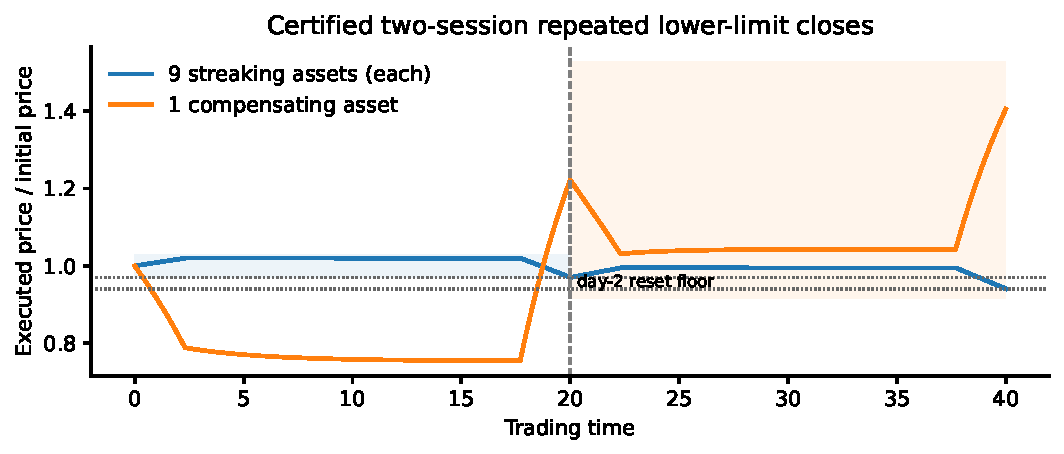
\includegraphics[width=0.87\linewidth]{figures/v7_certified_multiday_prices.pdf}
\caption{\textbf{An interval-certified two-session path.} Continuous target and compensator prices for the construction in Proposition~\ref{prop:certified-v7}. The nine targets close at the reset lower limits; the compensator stays inside its 25\% daily limits. Curves are illustrative numerical reconstructions; admissibility is independently certified by the outward-rounded arithmetic described in Appendix~\ref{app:v7certificate}.}\label{fig:v7path}
\end{figure}
Figure~\ref{fig:v7rates} displays the corresponding gross execution rates.

\begin{figure}[H]\centering
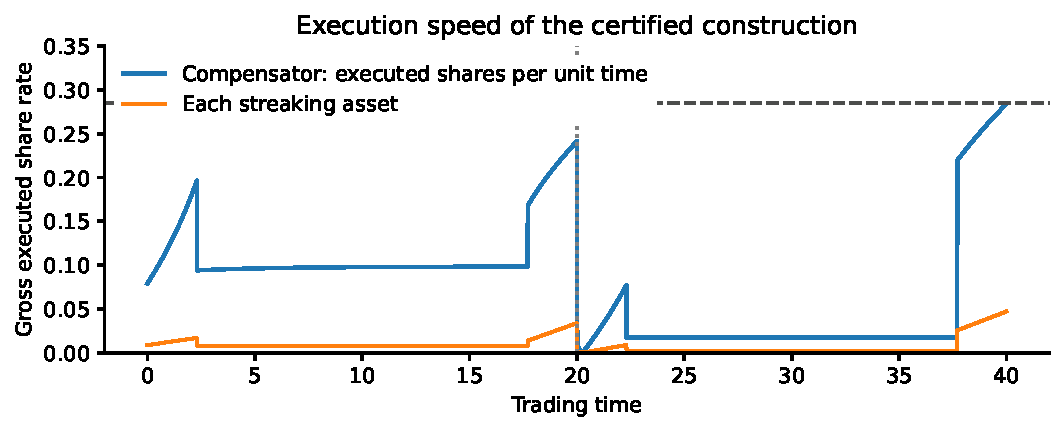
\includegraphics[width=0.87\linewidth]{figures/v7_certified_rate_path.pdf}
\caption{\textbf{Gross execution rates in the certified path.} The largest computed gross share-rate is approximately $0.28422$; rigorous interval rounding certifies a bound strictly below $0.285$, without instantaneous pulses. The cap is per asset, before netting buys and sells.}\label{fig:v7rates}
\end{figure}
\FloatBarrier


\subsection{Certified loss--breadth comparisons under uniform rolling bands}
\label{subsec:loss-breadth}
The preceding two-session witness fixes nine targets at
consecutive $3\%$ lower-band closes, with a single compensator
under a wider band. Here we compare additional feasible paths
under a \emph{different} model protocol: every asset receives
a symmetric $\pm25\%$ price band in each of two sessions, reset
at the preceding close. All rows retain $N=10$, $F=\eta=1$,
$\rho=0.4$, $T=40$ with two 20-unit sessions, a gross
per-asset share-rate cap of $0.285$, available sale shares
below $2$, and exact terminal dollar-ledger closure.

In each new case $k$ target assets follow an identical piecewise
constant executed-dollar rate $u(t)$, and the remaining $10-k$
assets follow $-ku(t)/(10-k)$. The inputs are exact rational
segments satisfying $\int_0^{40}u(t)\dd t=0$.
Integer outward-rounded interval enclosures certify both
group-price paths, entire rolling price bands, sale-rate and
inventory constraints, turnover, and a terminal geometric-index
loss bound. Details and complete inputs are in
Appendix~\ref{app:loss-breadth} and
\path{verification/loss_breadth_certified.py}.

\begin{table}[tbp]\centering\small
\caption{\textbf{Systemic loss--breadth comparison for specified
positive-price dollar-closed controls.} All new cases use uniform
two-session $\pm25\%$ rolling bands, unlike the original
$3\%$-target/$25\%$-compensator witness. Target loss denotes an
ordinary price decline in at least $k$ assets; index loss
denotes the decline of the equal-weight geometric price index.
Prefixes \texttt{P} and \texttt{R} identify, respectively,
two-window and three-window piecewise-constant trading templates;
the labels indicate coverage percentage and nominal target loss,
and \texttt{M5} denotes the relaxed $M<5$ budget. Loss
thresholds are conservative strict lower bounds, whereas the
$M$ and gross-rate columns give certified upper bounds.}
\label{tab:loss-breadth}
\begin{tabular}{@{}lrrrrrr@{}}\toprule
Witness & $k$ & Target loss & Index loss & $M$ upper &
\shortstack{Max. gross\\rate} & $M$ cap\\\midrule
Original & 9 & $5.91\%$ & $>1.98\%$ & $2.984$ & $0.284500$ & $3$\\
P50-20 & 5 & $>22.29\%$ & $>4.0\%$ & $2.600$ & $0.216130$ & $3$\\
P60-20 & 6 & $>20.90\%$ & $>5.0\%$ & $2.880$ & $0.257224$ & $3$\\
P70-10 & 7 & $>12.60\%$ & $>3.0\%$ & $2.660$ & $0.164249$ & $3$\\
R80-10 & 8 & $>10.80\%$ & $>3.0\%$ & $2.851$ & $0.272696$ & $3$\\
R70-15.5 & 7 & $>15.50\%$ & $>4.0\%$ & $2.940$ & $0.277592$ & $3$\\
R70-20-M5 & 7 & $>20.20\%$ & $>6.0\%$ & $4.600$ & $0.262743$ & $5$\\
\bottomrule\end{tabular}
\end{table}

\begin{proposition}[An eight-asset large drawdown under uniform rolling bands]
\label{prop:loss-breadth-eight}
Under the uniform $\pm25\%$ two-session protocol above, there exists
a positive-price, absolutely continuous paired-dollar path satisfying
$X_i(40)=0$ and $H_i^-<2$ for every asset, together with
\[
S_i(40)<0.892F\quad(1\le i\le8),\qquad
\Cris_{0.8}(40)>-\log(0.97),\qquad
M<3,\quad\bar v_{\rm used}<0.285.
\]
\end{proposition}
\begin{proof}
Under the exact rational schedule \texttt{R80-10}, the common
target price $x(t)$ and compensator price $y(t)$ satisfy
$\dot x=-0.4(x-1)+u(t)/x$ and
$\dot y=-0.4(y-1)-4u(t)/y$.
Outward-rounded fixed-point interval arithmetic
(Appendix~\ref{app:loss-breadth}) encloses both trajectories
on $[0,40]$ and verifies all rolling-band, rate, turnover,
and share-sale constraints. The certified endpoints satisfy
$x(40)<0.892$ and $x(40)^8y(40)^2<0.97^{10}$.
Finally, $\int_0^{40}u(t)\dd t=0$ ensures
$X_i(40)=0$ for every asset.
\end{proof}

As shown in the final row of Table~\ref{tab:loss-breadth},
the $70\%$-coverage control reaching a target decline above
$20.2\%$ uses paired-dollar turnover $M<4.600<5$.
Whether a different control can reach the same target with
$M\le3$ remains open.

\FloatBarrier

\section{Discussion and model extensions}\label{sec:discussion}
\subsection{Economic accounting and execution burden}
Recovery has two roles: for the price-level dynamics in Assumption~\ref{asmp:model}, it enters the curvature-based exclusion argument, but it also makes nontrivial terminal displacement possible under dollar closure. If $\rho=0$, $\dd\Phi(S_i)=\dd X_i$ and $X_i(T)=0$ implies $S_i(T)=F$ (Appendix~\ref{app:accounting}). For $\rho>0$, the identity \eqref{eq:cost} shows that the nonnegative terminal potential and cumulative recovery dissipation are financed by a reduction of net share inventory, valued at the fixed benchmark. For any terminally dollar-closed path $\gamma$, define this benchmark-valued inventory consumption by
\[
\mathcal K(\gamma):=
F\sum_i\bigl[\theta_i(0)-\theta_i(T)\bigr]
=\sum_i E(S_i(T))+
\rho\sum_i\int_0^T\frac{(S_i(t)-F)^2}{g(S_i(t))}\dd t\ge0.
\]
The functional $\mathcal K(\gamma)$ records the benchmark value of inventory consumed by terminal displacement and recovery dissipation. It uses dollar closure and accounts for net share-inventory consumption; transaction fees, spreads, outside funding, and counterparty balance sheets enter through additional costs. The inventory bound in Section~\ref{sec:budget} motivates an associated resource-minimization problem.

As a direct bound for the ten-asset certificate, $E(S)=(S-1)^2/2$ and the certified terminal compensator lower endpoint $y(40)>1.4047874$ give
\[
\mathcal K(\gamma)\ \ge\ \sum_i E(S_i(40))
>\frac92(1-0.9409)^2+\frac12(1.4047874-1)^2>0.0976.
\]
The certified terminal interval supplies this bound; enclosing the recovery integral would sharpen it. Let $\Gamma_{\alpha,\delta}$ denote the admissible paths satisfying the terminal crisis, pairing, closure, and execution restrictions. A natural extension is to optimize
\[
\mathcal K_{\min}(\alpha,\delta)
=\inf_{\gamma\in\Gamma_{\alpha,\delta}}\mathcal K(\gamma).
\]
Jointly minimizing this inventory cost, executed-dollar turnover, and the gross rate gives a constrained optimal-control problem.

\subsection{Dependence on resilience, impact, and the loss metric}
Our global elasticity conditions rely jointly on the local response $g$ and linear \emph{price-level} restoration toward $F$. Under volume displacement recovery as described in Section~\ref{sec:model}, $\dot\Phi|_{\mathrm{vol}}=-\rho S V(S)$ replaces the specific drift used in the tangent comparison; establishing elasticity barriers for that alternative model requires a separate curvature analysis. A more general theory would classify which restoring fields preserve analogous barrier regions. The elasticity $e(S)=Sg'(S)/g(S)$ differentiates local per-share impact with respect to the price state; cumulative metaorder impact instead depends on order size, execution history, and replenishment \citep{AlfonsiFruthSchied2010,BucciEtAl2019,CuratoGatheralLillo2017}.

The severity of Market C is also a boundary result: logarithmic loss diverges as a positive price tends to zero, while constant $g$ yields finite coordinate distance and finite inventory potential at that boundary. Fixed strictly positive price floors, realistic depth deterioration, rate caps, and trade halts can all limit its quantitative significance without invalidating the mathematical existence theorem. Accordingly, the attainable-loss bounds in Section~\ref{sec:rateband} describe the quadratic small-rate regime; reaching a fixed large threshold requires adequate execution capacity.

The definition $\Cris_\alpha=\min\{\overline L,Q_\alpha\}$ uses the equal-weight geometric price index as well as coverage. Metric choice matters: in the $p=1$ market, paired-dollar trades give $\dd\sum_i S_i|_{\rm trade}=(\eta/F)\sum_i\dd X_i=0$, and the common price-level recovery preserves the initial sum $NF$. Thus the arithmetic mean remains $F$ even when a partial-coverage geometric-index crisis is reachable. Market-capitalization-weighted indices, arithmetically aggregated prices, rolling-peak losses, and different coverage criteria define different target sets. Changing the weighting or loss baseline changes the corresponding target set for reachability.

\subsection{What the two-session certificate establishes}
The construction in Proposition~\ref{prop:certified-v7} is a constrained \emph{existence witness} for one specified ten-asset market. Nine equal target prices lose $5.91\%$ over two sessions, while the receiving asset has a high-precision reconstructed final price near $1.40516 F$. The equal-weight geometric-index decline is approximately $2.06\%$ (the mean log loss is approximately $0.02081$), whereas the arithmetic mean price decreases by only about $1.27\%$. The receiving asset supports large temporary price excursions within its wider rolling band. Table~\ref{tab:sensitivity} varies composition \emph{holding the control fixed}, rather than optimizing a new control for each $k$.

The gap in the bracket $0.044<\bar v_*<0.285$ reflects the distance between a general analytical lower bound for the fixed model parameters and a specific feasible trajectory. The certificate rigorously verifies pathwise constraints and ledger closure, establishing that the admissible trajectory set is nonempty under stylized $3\%$ target bands and $25\%$ compensator bands. The Tokyo Stock Exchange sets daily limits as tiered \emph{absolute yen} amounts based on reference prices and conditionally widens them after specified limit-bound sessions with little or no execution \citep{JPX2026}. Research on actual price-limit regimes provides an institutional comparison to the proportional-reset protocol used here \citep{KimRhee1997,Chen2019}.

\subsection{Further directions}
Nonlinear recovery operators raise the question of which restoring fields preserve the $\Phi$-based invariant regions. General heterogeneous $(g_i,\rho_i,F_i)$, changing network topology, and nonseparable cross-impact alter the scalar potential argument; Subsection~\ref{subsec:barrier-robustness} establishes one diagonal extension with common $F$ and $\rho$. For invertible matrix impact $\dd\bm S=\mathsf G(\bm S)\dd\bm\theta$, an additive transaction potential would depend on exactness of the one-form
\[
\omega=\one^\top\operatorname{diag}(\bm S)\mathsf G(\bm S)^{-1}\dd\bm S
\]
and on the compatible sign of its restoring drift. Matrix symmetry alone is not sufficient. Cross-impact no-dynamic-arbitrage restrictions \citep{AlfonsiKlockSchied2016,SchneiderLillo2019} and empirical multivariate impact \citep{BenzaquenEtAl2017} provide separate benchmarks.

Joint optimization of inventory cost, turnover, and the minimum feasible gross rate would connect reachability with trading incentives, including strategic predation \citep{BrunnermeierPedersen2005}. Proposition~\ref{prop:turnover-dissipation} aggregates across assets and does not use per-asset terminal dollar closure. When $X_i(T)=0$, the constant-impact dynamics also give the subset-level identity
\[
\frac{F^2-S_i(T)^2}{2}
=\rho\int_0^T S_i(t)(S_i(t)-F)\dd t
\qquad\text{for every }i.
\]
This identity isolates each falling asset and may yield tighter subset-level turnover bounds. The squared-price dynamics,
$\dd(S_i^2)=-2\rho S_i(S_i-F)\dd t+2\eta\dd X_i$,
also have a trade term without the denominator $1/S_i$; their restoring drift remains nonlinear. An upper price bound $S_i\le U_{\max}$ together with the gross share-rate cap gives
$\dot M\le NU_{\max}\bar v/2$. For fixed positive turnover, this prevents concentration at the single peak of the time kernel in~\eqref{eq:V2-turnover} and permits a tighter weighted-turnover estimate. These constraints suggest time-dependent resource bounds sensitive to the composition of selling and receiving assets. Empirical identification of local impact $g$, recovery, trade direction, and accessible inventories would require time-resolved transaction and order-book observations; market-microstructure invariance~\citep{KyleObizhaeva2023} provides a scaling benchmark. A stochastic flow or equilibrium-selection model could then place probabilities alongside the present deterministic reachability results.

\subsection{Robustness to unmatched dollar flow and impact heterogeneity}
\label{subsec:barrier-robustness}
The exclusion in Theorem~\ref{thm:barrier2} uses both a common
price-response function and exact dollar pairing. The local logarithmic
price response per executed dollar is
$\lambda(S)=g(S)/S^2$, with elasticity
\[
\frac{\dd\log\lambda(S)}{\dd\log S}=e(S)-2.
\]
Thus the threshold $e\ge2$ states that this model's local
per-dollar log-impact does not increase as the price falls.
We quantify two departures from the hypotheses of the exclusion theorem
while retaining fixed fundamentals and common price-level recovery.

\begin{proposition}[Stability under unmatched dollar flow]
\label{prop:unbalanced-stability}
Suppose $S_i(0)=F$, all prices remain positive, and the homogeneous
response $g>0$ and common recovery rate $\rho>0$ satisfy
$e(S)\ge2$ on an interval containing $F$ and every attained price.
For absolutely continuous executed-dollar flows, relax exact pairing
to $\sum_i\dot X_i(t)=\varepsilon(t)$ with
$\varepsilon\in L^1([0,T])$. Then, for all $t\in[0,T]$ and
$\alpha\in(0,1]$,
\[
\begin{aligned}
\Cris_\alpha(t)\le\overline L(t)
&\le-\frac{g(F)}{NF^2}
 \int_0^t e^{-\rho(t-s)}\varepsilon(s)\,\dd s\\
&\le\frac{g(F)}{NF^2}
 \int_0^t e^{-\rho(t-s)}[-\varepsilon(s)]_+\,\dd s.
\end{aligned}
\]
\end{proposition}
\begin{proof}
Let $H(t)=\sum_i\Phi(S_i(t))$, where $\Phi(F)=0$
and $\Phi'(S)=S/g(S)$. Concavity of $\Phi$, implied by
$e\ge2$, gives $(S-F)\Phi'(S)\le\Phi(S)$. Hence
\[
\dot H=\varepsilon-\rho\sum_i(S_i-F)\Phi'(S_i)
\ge\varepsilon-\rho H,
\]
and $H(0)=0$ implies
$H(t)\ge\int_0^t e^{-\rho(t-s)}\varepsilon(s)\,\dd s$.
Moreover, $G(q)=\Phi(Fe^q)$ is concave and
$G'(0)=F^2/g(F)$, so its tangent inequality yields
\[
H(t)=\sum_iG(q_i(t))
\le\frac{F^2}{g(F)}\sum_iq_i(t)
=-\frac{NF^2}{g(F)}\overline L(t).
\]
Combining these bounds and discarding the nonnegative part of
$\varepsilon$ in the weighted integral proves the claim.
\end{proof}

Here $\varepsilon$ measures the unmatched executed-dollar rate
\emph{within the selected asset set}; it need not represent a net
cash flow into the wider market. Exact pairing recovers
Theorem~\ref{thm:barrier2}. The estimate does not require
terminal dollar-ledger closure.

\begin{proposition}[Weighted-flow bound for heterogeneous quadratic impact]
\label{prop:heterogeneous-quadratic}
Suppose $S_i(0)=F$ and
$g_i(S)=\eta_i(S/F)^2$, where $\eta_i>0$, with common
$F>0$ and $\rho>0$. For positive absolutely continuous
trajectories set $\kappa_i=\eta_i/F^2$ and
$\omega(t)=\sum_i\kappa_i\dot X_i(t)$.
Then, for all $t\in[0,T]$ and $\alpha\in(0,1]$,
\[
\begin{aligned}
\Cris_\alpha(t)\le\overline L(t)
&\le-\frac1N\int_0^t e^{-\rho(t-s)}\omega(s)\,\dd s\\
&\le\frac1N\int_0^t e^{-\rho(t-s)}[-\omega(s)]_+\,\dd s.
\end{aligned}
\]
Writing $\bar\kappa=N^{-1}\sum_i\kappa_i$ and
$\varepsilon=\sum_i\dot X_i$, the weighted imbalance decomposes as
\[
\omega=\bar\kappa\,\varepsilon+
\sum_i(\kappa_i-\bar\kappa)\dot X_i.
\]
Consequently exact dollar pairing alone need not eliminate the
weighted flow when the impact strengths differ.
\end{proposition}
\begin{proof}
With $q_i=\log(S_i/F)$, the impact law becomes
$\dot q_i=-\rho(1-e^{-q_i})+\kappa_i\dot X_i$.
Jensen's inequality and $e^x\ge1+x$ imply
\[
\begin{aligned}
\frac{\dd}{\dd t}\overline L(t)
&=\rho\left(1-\frac1N\sum_i e^{-q_i}\right)
-\frac{\omega}{N}\\
&\le\rho(1-e^{\overline L})-\frac{\omega}{N}
\le-\rho\overline L-\frac{\omega}{N}.
\end{aligned}
\]
The result follows by comparison from $\overline L(0)=0$.
\end{proof}

\paragraph{A terminally dollar-closed counterexample}
The loss of the homogeneous barrier is possible even with
exact dollar pairing \emph{and} terminal closure. Take $N=2$,
$\kappa_1>\kappa_2>0$, and two matched executed-dollar pulses:
$(\dd X_1,\dd X_2)=(a,-a)$ at time $0$, followed by
$(-a,a)$ at time $T>0$. Both asset ledgers close exactly,
and total paired-dollar turnover is $2a$.
Writing $r=e^{-\rho T}\in(0,1)$, the terminal log prices are
\[
\begin{aligned}
q_1(T)&=\log\bigl(1+r(e^{\kappa_1a}-1)\bigr)-\kappa_1a,\\
q_2(T)&=\log\bigl(1+r(e^{-\kappa_2a}-1)\bigr)+\kappa_2a.
\end{aligned}
\]
For sufficiently small $a>0$, Taylor expansion gives
\[
\overline L(T)=
\frac{(1-r)(\kappa_1-\kappa_2)}2\,a+O(a^2)>0,
\qquad
Q_{1/2}(T)=(1-r)\kappa_1a+O(a^2)>0.
\]
Therefore $\Cris_{1/2}(T)>0$, although each response has
elasticity $e_i=2$. Prices remain strictly positive, and a
sufficient initial share inventory covers the finite sales.
This is a pulse-admitting construction, without an instantaneous
gross-rate cap. The common-impact hypothesis of Theorem~\ref{thm:barrier2}
fails in this example.

The two perturbation estimates isolate departures from matching
and homogeneous impact strength. They keep $F$ and $\rho$ fixed;
time-varying fundamentals, heterogeneous restoration, and
nonseparable cross-impact require separate analysis.

\section{Conclusion}\label{sec:conclusion}
For a specified price-level resilience and paired-dollar execution protocol, the response-adapted coordinate identifies global barriers, feasible partial-coverage regimes, and a sharp full-coverage ceiling. Necessary dollar turnover and inventory are conveniently expressed in the generalized price coordinate and in units of local benchmark impact. The uniform finite-resource severe partial-coverage construction extends from constant impact to every fixed exponent $0\le p<1$ in the power-law family, with resource constants that may deteriorate as $p\uparrow1$. For constant impact on a bounded positive-price region, executed-dollar turnover also bounds the terminal quadratic price-potential deficit. A finite gross-rate cap changes the scale of attainable small systemic losses, and one independently interval-certified two-session witness satisfies the simultaneous rate, band, and dollar-ledger requirements. The economic accounting identity makes explicit the benchmark-valued inventory consumed by dollar-closed price pressure. Perturbation bounds identify the effects of unmatched dollar flows and heterogeneous quadratic impact on the elasticity barrier. Together, these results clarify the structural and resource boundaries of liquidity-driven drawdowns within a deterministic execution framework. Alternative resilience laws, heterogeneous cross-impact and minimum-cost controls offer distinct mathematical directions for future work.

\section*{Code and numerical data availability}
The research code, numerical data, certificates, and reproduction instructions are publicly available at \url{https://github.com/Siyuan-chat/market-crash-reachability}. The unchanged original computational baseline is associated with \href{https://github.com/Siyuan-chat/market-crash-reachability/tree/ea831c44f5b77b7039dd6644f6f0a791bb74d176}{commit \texttt{ea831c4}}; the frozen software archive is separately identified by \href{https://doi.org/10.5281/zenodo.23428183}{DOI 10.5281/zenodo.23428183}. Appendices~\ref{app:v7certificate} and~\ref{app:loss-breadth}
describe the two families of interval certificates and their
verification scripts; Appendix~\ref{app:sublinear-severe}
provides the constructive proof for sublinear impact. Reproduction commands and software requirements are in \path{REPRODUCE.md}; the checksum manifest is \path{release/SHA256SUMS}. The underlying certificate was previously regenerated from source, with independent floating-point ODE and exact-rational consistency checks.

\section*{Declaration on AI-assisted tools}
AI-assisted tools were used for language editing, manuscript organization, and assisting with verification and figure-generation scripts. The author takes full responsibility for all mathematical proofs, numerical certificates, and scientific content.

\appendix
\section{Settlement, coordinate changes, and variation bounds}\label{app:accounting}
The continuous response rule is interpreted along finite-variation execution paths. During an idealized pulse, physical time is frozen ($\dd t=0$) and the states move along the response ODE as the executing share size varies. The pulse's executed dollar transfer is the \emph{integral} $\int S_i\dd\theta_i$, not the beginning-of-pulse price times the final share increment. By continuity of $g>0$, its endpoints can be joined by an admissible response path whenever the intervening price stays positive.

For one asset the differential rule reads
\begin{equation}\label{eq:appendix-s}
\dd\theta=\frac{\dd S+\rho(S-F)\dd t}{g(S)}.
\end{equation}
Decompose $S=F+(S-F)$ and integrate:
\begin{align*}
\int_0^T S\dd\theta
&=F[\theta(T)-\theta(0)]
+\int_F^{S(T)}\frac{u-F}{g(u)}\dd u
+\rho\int_0^T\frac{(S-F)^2}{g(S)}\dd t,
\end{align*}
where the initial price is $F$. This proves \eqref{eq:cost}. For $S<F$ the primitive $E(S)$ in \eqref{eq:E} is also nonnegative because the integration orientation reverses the sign of the negative integrand. Hence if $\theta(T)=\theta(0)$, the total executed cost cannot be negative.

Let $y=\Phi(S)$ and $z=\Psi(S)$, with
\[
\Phi'(S)=\frac{S}{g(S)},\qquad \Psi'(S)=\frac1{g(S)}.
\]
Then
\begin{equation}\label{eq:appendix-yz}
\dd y=\dd X-\rho\frac{S(S-F)}{g(S)}\dd t,
\qquad
\dd z=\dd\theta-\rho\frac{S-F}{g(S)}\dd t.
\end{equation}
The recovery terms have signs opposite to $S-F$. Thus whenever $y<0$ (equivalently $S<F$), the no-trade drift in $y$ is positive; likewise for $z$. By separating the positive and negative variations in \eqref{eq:appendix-yz}, a trajectory ending at $y(T)\le\Phi(s)<0$ must accumulate at least $-\Phi(s)$ in negative executed-dollar variation. One way to see this is to start at the \emph{last} time when $y$ equals zero (or $t=0$ if no later zero exists). On the remaining interval $y\le0$ and the recovery drift is nonnegative. The negative transaction variation must therefore account for the entire fall to $y(T)$. The same argument in $z$ gives the share-sale bound. Summing sales across qualifying assets counts each paired-dollar transfer at most once. If a terminally qualifying asset has inventory cap $H_i$ and $X_i(T)=0$, equation \eqref{eq:cost} implies
\[
E(S_i(T))\le F\left[\theta_i(0)-\theta_i(T)\right]\le FH_i.
\]
Since $E(S)$ increases as $S$ falls below $F$, $S_i(T)\le s$ implies $E(s)\le FH_i$. This proves Theorem~\ref{thm:resource}.

When $\rho=0$, $\dd\Phi(S_i)=\dd X_i$. Terminal dollar closure therefore implies $\Phi(S_i(T))=\Phi(F)=0$ and, by strict monotonicity, $S_i(T)=F$. Within the present separable response class, recovery makes the nontrivial dollar-closed endpoint effect possible.

\section{Local two-pulse and three-pulse expansions}\label{app:local}
We document the expansion used in Propositions~\ref{prop:two-pulse} and \ref{prop:three-pulse}. Normalize local variations by $x=S/F-1$ and $c=g(F)/F^2$. At $S=F$, the executed-dollar coordinate $y=\Phi(S)$ satisfies $\Phi(F)=0$, $\Phi'(F)=F/g(F)$, and
\begin{equation}\label{eq:local-inverse}
\frac{\dd S}{\dd y}=\frac{g(S)}S,
\qquad
\frac{\dd^2 S}{\dd y^2}=
\frac{g(S)[Sg'(S)-g(S)]}{S^3}.
\end{equation}
Hence, writing $e_0=e(F)$, the price ratio after a small dollar-coordinate displacement $y$ is
\begin{equation}\label{eq:local-Taylor}
\frac SF=1+cy+\frac12(e_0-1)c^2y^2+O(y^3),
\end{equation}
with constants uniformly bounded for paths in a compact neighborhood of $F$.

For the two-pulse experiment, the first impulse displaces $y$ by $hu_i$ at time zero. It produces the initial price response according to \eqref{eq:local-Taylor}. Recovery over $T$ multiplies the \emph{level} displacement $S-F$ by $r=e^{-\rho T}$; the terminal pulse subtracts the same dollar amount $hu_i$ from the executed-dollar coordinate. Expanding $\Phi$ and $\Phi^{-1}$ around $F$ gives
\begin{align}\label{eq:local-two}
L_i(T)&=c(1-r)hu_i+\frac{c^2h^2}{2}\,\lambda(r,e_0)u_i^2+O(h^3),\\
\frac1N\sum_i L_i(T)&=\frac{c^2h^2}{2N}(1-r)(2-e_0-r)\sum_i u_i^2+O(h^3),\nonumber
\end{align}
where the individual second-order coefficient $\lambda$ is not needed separately. The linear term vanishes in the mean because $\sum_i u_i=0$. If at least $k$ components are positive, those assets have positive first-order losses and the $k$th-largest loss is positive for small $h$; the mean is positive under the stated time-curvature condition.

For the three-pulse experiment, the dollar-coordinate impulses at $0,T/2,T$ have amounts $hu_i$, $-(1+r)hu_i$, and $rhu_i$ with $r=e^{-\rho T/2}$. Direct substitution and second-order expansion yield
\begin{equation}\label{eq:local-three}
L_i(T)=\frac{1-e_0}{2}c^2h^2u_i^2r(1-r^2)+O(h^3),
\end{equation}
with first-order terms canceling exactly. If $e_0<1$ and every $u_i\ne0$, all terminal losses are positive for sufficiently small $h$. Since every pulse amount vector is zero-sum and the amounts cancel componentwise over the full horizon, the construction also satisfies the paired-dollar and terminal dollar-closure rules. The initial inventory requirement and turnover are finite for fixed $h$.

\section{Uniform-resource severe drawdowns for partial coverage}\label{app:severe}
We prove Theorem~\ref{thm:ABC}(C) constructively. Fix $N\ge2$, set $m=N-1$, and choose the constant-response model $g(S)=\eta>0$. We may assume the target crisis threshold $\delta$ is large, since a path exceeding a larger threshold automatically exceeds every smaller one. It is enough to produce $m$ terminal prices $\varepsilon\downarrow0$ with one remaining compensator asset, because every $k<N$ satisfies $k\le m$.

\subsection{A radial representation of paired-dollar trading}
For $g\equiv\eta$,
\begin{equation}\label{eq:radius-appendix}
\dd(S_i^2)= -2\rho S_i(S_i-F)\dd t+2\eta\dd X_i,
\qquad \one^\top\dd\bm X=0.
\end{equation}
Let $R=(\sum_iS_i^2)^{1/2}$. A paired-dollar trade keeps $R$ fixed; a positive-price change at fixed $R$ is implementable as a finite-variation path in the positive orthant of that sphere. In particular, interpolate the squared prices $Y_i=S_i^2$ linearly between two positive vectors of the same sum: every intermediate $Y_i>0$ and $\sum_i\dd Y_i=0$, so $\dd X_i=\dd Y_i/(2\eta)$ is an admissible paired-dollar transfer. The corresponding share increment is $\dd\theta_i=\dd S_i/\eta$.

Fix $\beta=1/5$. Choose $c>0$ sufficiently small that, for every $b\in[0,\beta]$, the quantities
\begin{equation}\label{eq:abcs}
a=\sqrt{1-b^2-(m-1)c^2},\qquad H=a+(m-1)c+b
\end{equation}
satisfy $a>\max\{b,c\}$ and $bH<1$. For example, $0<c<1/(10m)$ suffices. The constructed path uses $b\in(0,\beta)$; the endpoint $b=0$ is used only by continuous extension in the root-bracketing argument below. During stage $j\in\{1,\dots,m\}$, fix the spherical direction
\begin{equation}\label{eq:uj}
\bm u_j=(c,\ldots,\underbrace{a}_{j},\ldots,c,b),
\qquad \|\bm u_j\|_2=1.
\end{equation}
Set $\bm S(t)=R(t)\bm u_j$ throughout the stage. To make it solve the price equations, use
\begin{equation}\label{eq:R}
R(t)=F\left[H+(\sqrt N-H)e^{-\rho t}\right],
\qquad
\dot\theta_i=\frac{\rho F}{\eta}\left(u_{j,i}H-1\right).
\end{equation}
Indeed, differentiating $S_i=u_{j,i}R(t)$ in the price equation gives \eqref{eq:R} and
\begin{equation}\label{eq:dXdt}
\dot X_i=\frac{\rho FR(t)}\eta\,u_{j,i}(u_{j,i}H-1),
\quad \sum_i\dot X_i=\frac{\rho FR(t)}\eta\left(H\sum_i u_{j,i}^2-\sum_i u_{j,i}\right)=0,
\end{equation}
because $\sum_i u_{j,i}^2=1$ and $\sum_i u_{j,i}=H$.

\subsection{Closing the compensator's dollar flow}
At $t=0$ begin with $F\one$ and apply a positive-price pulse at fixed radius $F\sqrt N$ to the first direction $\bm u_1$. Switch between stages $\bm u_j$ using similar fixed-radius pulses. At time $T$ use a final fixed-radius pulse to reach
\begin{equation}\label{eq:endpoint-severe}
S_1(T)=\cdots=S_m(T)=\varepsilon,
\quad S_N(T)=\sqrt{R(T)^2-m\varepsilon^2}.
\end{equation}
The terminal price vector is positive for all sufficiently small $\varepsilon$.

For constant $g$, integrating \eqref{eq:radius-appendix} gives the exact executed-dollar ledger
\begin{equation}\label{eq:Xledger}
X_i(T)=\frac{S_i(T)^2-F^2}{2\eta}
+\frac\rho\eta\int_0^T S_i(t)[S_i(t)-F]\dd t.
\end{equation}
For the compensator, its stage weight is always $b$. Define
\begin{align}\label{eq:compensator}
\mathcal F_\varepsilon(b)=\frac{R_b(T)^2-m\varepsilon^2-F^2}{2\eta}
+\frac\rho\eta\int_0^T bR_b(t)[bR_b(t)-F]\dd t,
\end{align}
where $R_b$ depends continuously on $b$ through \eqref{eq:R}. With $c$ fixed, choose a sufficiently large finite $T$ such that $\mathcal F_0(\beta)<0$. Such a choice exists because $R_\beta(t)\to FH_\beta$ and $\beta H_\beta<1$: the integral in~\eqref{eq:compensator} then has a strictly negative linear term in $T$, while the terminal term remains bounded. Here $H_\beta$ denotes $H$ evaluated at $b=\beta$. Fix this horizon. Since $R_0(T)>F$, we have $\mathcal F_\varepsilon(0)>0$ for all sufficiently small $\varepsilon>0$, whereas
\[
\mathcal F_\varepsilon(\beta)=\mathcal F_0(\beta)-\frac{m\varepsilon^2}{2\eta}<0.
\]
Continuity therefore gives $b(\varepsilon)\in(0,\beta)$ for which
\[
X_N(T)=\mathcal F_\varepsilon(b(\varepsilon))=0.
\]
Both $c$ and $T$ are fixed independently of $\varepsilon$.

\subsection{Closing every target asset's dollar flow}
It remains to make the other $m$ terminal dollar balances equal. Whenever an asset is in the high state $a$ rather than the low state $c$, the difference in its recovery integrand is
\begin{equation}\label{eq:W}
W(t)=(a-c)R(t)\big[(a+c)R(t)-F\big].
\end{equation}
This is strictly positive: $(a+c)H=1+b(a-b)+mac+bc>1$, and $R(t)\ge FH$. Consequently $W(t)>0$ for $t\in[0,T]$. Choose a partition $0=t_0<\dots<t_m=T$ such that
\begin{equation}\label{eq:weights}
\int_{t_{j-1}}^{t_j}W(t)\dd t=\frac1m\int_0^T W(t)\dd t,
\qquad j=1,\ldots,m.
\end{equation}
The continuous, strictly increasing cumulative integral makes this partition possible. Let target asset $j$ occupy the high state in stage $j$ and the low state otherwise. All target assets have the same initial price $F$, terminal price $\varepsilon$, and recovery integral in \eqref{eq:Xledger}, hence identical terminal balances $X_i(T)$. Every pulse and every stage respects $\sum_i\dd X_i=0$; since $X_N(T)=0$, the common target balance must also vanish. Therefore
\begin{equation}\label{eq:allclosed}
X_i(T)=0\qquad\text{for every } i=1,\ldots,N.
\end{equation}

\subsection{Uniform finite turnover and inventory}
The path remains in the positive sphere of radius at most $F\sqrt N$, so $0<S_i\le F\sqrt N$ throughout. There are $m+1=N$ fixed-radius pulses, and each pulse can be implemented by monotone componentwise interpolation in squared-price coordinates. Consequently the cumulative paired-dollar pulse turnover has an explicit, though loose, upper bound depending only on $N,F,\eta$. For example, a safe bound is $N^3F^2/(4\eta)$. During recovery-controlled stages, $\sum_i|\dot X_i|/2\le \rho NF^2/\eta$, giving
\begin{equation}\label{eq:uniformM}
M(\gamma)\le M_0:=\frac{N^3F^2}{4\eta}+\frac{\rho NF^2T}{\eta}.
\end{equation}
Likewise, share sales over $N$ pulses plus the continuous stages are bounded by
\begin{equation}\label{eq:uniformH}
H_i^-\le H_0:=\frac{NF\sqrt N+\rho FT(\sqrt N+1)}\eta,
\end{equation}
independently of $\varepsilon$. Starting with at least $H_0$ shares of each asset rules out short sales. The compensator's price stays bounded and positive; its log loss remains finite. The other $m$ losses are $\log(F/\varepsilon)\to\infty$. Hence their $k$th order statistic and the average loss both diverge when $k\le m$. Thus $\Cris_\alpha(T)\to\infty$ with fixed finite $M_0,H_0$, proving Theorem~\ref{thm:ABC}(C).\qed

\section{Construction proving the sharp full-coverage bound}\label{app:sharp}
The necessary radial inequality was established in the proof of Theorem~\ref{thm:critical}. For sufficiency, we construct an admissible family approaching the bound. Fix $0<b<1/\sqrt N$, and choose
\begin{equation}\label{eq:fullab}
a=\sqrt{1-(N-1)b^2}>b,
\quad H=a+(N-1)b,
\quad R_b(t)=F\left[H+(\sqrt N-H)e^{-\rho t}\right].
\end{equation}
Use the $N$ positive unit-vector directions given by permutations of $(a,b,\ldots,b)$. At time zero pulse from $F\one$ to $R_b(0)\bm u_1$, then follow $S_i(t)=u_{j,i}R_b(t)$ using the same paired controls as in \eqref{eq:R}. When changing directions, use finite fixed-radius positive squared-price pulses. At time $T$, make a final pulse to the equal-price point
\begin{equation}\label{eq:fullend}
S_i(T)=\frac{R_b(T)}{\sqrt N},\qquad i=1,\ldots,N.
\end{equation}
For the recovery integrals to be identical for every asset, define
\begin{equation}\label{eq:fullW}
W_b(t)=(a-b)R_b(t)\big[(a+b)R_b(t)-F\big].
\end{equation}
Here $(a+b)H=1+Nab>1$, so $W_b(t)>0$ for $t\in[0,T]$. Split the interval into $N$ parts with equal integrals of $W_b$. In each part a different asset is the sole high-price coordinate. All $N$ assets now have the same initial price, the same terminal price, and the same recovery integral in \eqref{eq:Xledger}. Their final dollar balances are therefore identical; since all trades are paired, their sum is zero and each balance is exactly zero.

As $b\downarrow0$, the terminal equal price in \eqref{eq:fullend} tends to
\[
\frac{F}{\sqrt N}\left[1+(\sqrt N-1)e^{-\rho T}\right],
\]
whereas $b\uparrow1/\sqrt N$ yields $S_i(T)\to F$. Continuity in $b$ implies that every strictly intermediate common terminal price is reachable by a positive-price, finite-turnover, fully dollar-closed path. The corresponding log-loss range is precisely $0<\delta<\delta_{\rm crit}(N,T)$, completing the sharpness proof. The endpoint $\delta_{\rm crit}$ itself would require the limiting direction with zero components and is excluded by strict price positivity.\qed

\section{Bounded-rate control: analytic details and audit protocol}\label{app:rate}
For the three-bin control~\eqref{eq:bounded-control}, the identities $\int f=0$ and $\int e^{-\rho(T-t)}f(t)\dd t=0$ follow from equal bin widths and the geometric ratio $r=e^{-\rho T/3}$. Write $h_0=g(F)/F$ and $h_1=g(F)(e_0-1)/F^2$. The perturbation equations are $y'=-\rho y+h_0 f$, $z'=-\rho z+h_1fy$. Since $y(0)=y(T)=0$ and $(e^{-\rho(T-t)})'=\rho e^{-\rho(T-t)}$, one integration by parts gives the exact identity
\begin{equation}\label{eq:ibp}
\int_0^T e^{-\rho(T-t)}f(t)y(t)\dd t
=\frac{\rho}{2h_0}\int_0^T e^{-\rho(T-t)}y(t)^2\dd t.
\end{equation}
The resulting coefficient is $\rho/2$. Substituting $h_1/h_0=(e_0-1)/F$ and $L_i=-\log(S_i/F)$ proves~\eqref{eq:finite-rate-coefficient}. At $p=1$ the quadratic coefficient vanishes; this is consistent with the all-asset barrier but does not exclude a partial-coverage loss under a different bounded signal. The independent verifier integrates the nonlinear ODE directly with the dollar-rate signal, computes gross share execution before netting, and compares the finite-amplitude loss with~\eqref{eq:finite-rate-coefficient}.

A high-precision reconstruction of the severe pulse construction confirms its terminal-dollar accounting. Bounded-rate controls constitute a more restrictive admissible class, whose local construction and barrier are established separately.

\section{Numerical experiments and reproducibility}\label{app:numerics}
This appendix documents deterministic price paths constructed under the exact marginal-price settlement protocol. For the severe-crash construction we use $g(S)=1$, $F=\eta=\rho=1$. The code selects a positive price direction and numerically solves for the compensator direction and time partitions; between switches the radius and ledger have analytic primitives. At every transaction time the paired executed-dollar sum is zero, and at maturity \emph{each} signed-dollar ledger closes to numerical accuracy.

\begin{table}[H]\centering\small
\caption{Constructed paths with severe partial-coverage losses. The reported turnover is sufficient for these paths; the minimum turnover is unknown. All rows use target log loss $L=5$ and parameters normalized to unity.}\label{tab:witness}
\begin{tabular}{@{}rrrrrr@{}}\toprule
$N$ & $k$ & $T$ & $\mathcal C_\alpha(T)$ & Turnover $M$ & Max. sale shares \\\midrule
3 & 2 & 3 & 3.3168 & 2.6179 & 3.9320\\
12 & 11 & 4 & 4.5781 & 38.6861 & 8.0804\\
20 & 19 & 5 & 4.7477 & 104.1750 & 10.1906\\
\bottomrule\end{tabular}
\end{table}


Table~\ref{tab:target-loss} reports the effect of increasing the target log loss for $N=3$, $k=2$, and $T=3$.
\begin{table}[H]\centering\small
\caption{Effect of increasing target log loss for the fixed $N=3$, $k=2$, $T=3$ construction.}\label{tab:target-loss}
\begin{tabular}{@{}rrrr@{}}\toprule
Target log loss $L$ & Systemic loss $\Cris_{2/3}(T)$ & Turnover $M$ & \shortstack{Maximum cumulative\\share sales}\\\midrule
$3$ & $1.9845$ & $2.6128$ & $3.9365$\\
 $5$ & $3.3168$ & $2.6179$ & $3.9320$\\
$10$ & $6.6501$ & $2.6179$ & $3.9319$\\
$20$ & $13.3168$ & $2.6179$ & $3.9319$\\
\bottomrule\end{tabular}
\end{table}
The plotted experiment uses a finite, high-resolution sampling grid only to display continuous recovery segments; the underlying segment values and cash-flow integrals are evaluated using analytic expressions, and terminal closure is checked separately. For the $N=12$, $L=5$ construction, the maximum terminal dollar-ledger residual under double precision is less than $10^{-13}$ in the distributed script. Numerical tolerance is evidence of correct accounting implementation, not a substitute for the constructive proof in Appendix~\ref{app:severe}.

The numerical panels use model-generated inputs. Implementation details and reproduction commands are provided in the repository documentation.


\section{A reproducible interval certificate for the two-day construction}\label{app:v7certificate}
The certificate uses outward-rounded fixed-point intervals and Taylor enclosures, following standard validated-numerics principles \citep{Tucker2011}. The implementation \path{verification/certify_streak_interval.py} uses integer and rational arithmetic at scale $Q=10^{32}$, corresponding to resolution $Q^{-1}$; every multiplication and division is rounded outwards. The rational endpoint bracket for $h$ in~\eqref{eq:v7-root} has strictly opposite polynomial signs and the polynomial is strictly increasing on that bracket, so it contains the unique relevant exact root.

On each linear target segment, write $x(t)=a+vt$ in local segment time and $u(t)=x(t)[v+\rho(x(t)-1)]$. The compensator equation is the scalar nonautonomous ODE $\dot y=f(t,y):=-\rho(y-1)-9u(t)/y$. Its derivatives away from the finite set of target slope-change times are
\[
f_y=-\rho+\frac{9u}{y^2},\qquad f_t=-\frac{9u'}y,\qquad
 y''=f_t+f_y f,\qquad u'=v[v+\rho(2x-1)].
\]
The exact target plateaus and slopes yield conservative whole-segment enclosures $|u|<0.107$ and $|u'|<0.041$. On the bootstrap strip $0.70\le y\le1.60$, these imply $|f|<1.70$ and
\[
|y''|\le\frac{9|u'|}{0.70}
+\left(\rho+\frac{9|u|}{0.70^2}\right)
\left(0.60\rho+\frac{9|u|}{0.70}\right)<5.
\]
A tighter value of this last bound is recomputed with outward-rounded rational arithmetic on each of the six target segments. On a fixed grid of $h_0=1/2000$, a scalar comparison principle is combined with the one-step Taylor enclosure
\[
 y(t+h_0)\in y(t)+h_0 f(t,y(t))+[-B_j h_0^2/2,B_j h_0^2/2],
\]
where $B_j$ is the certified segment remainder bound. If the beginning state belongs to $[l,u]$, comparison of scalar ODE solutions gives the next lower bound from $l+h_0 f(t,l)-B_jh_0^2/2$ and the upper bound from $u+h_0 f(t,u)+B_jh_0^2/2$, each rounded outwards. A local $|f|<1.70$ excursion bound encloses the solution between grid points and verifies, inductively, that it stays in the bootstrap strip. The bound is reinitialized at each piecewise-linear slope discontinuity without taking an artificial step across it.

There are exactly $80,000$ certified grid steps. For the path in Proposition~\ref{prop:certified-v7}, the machine-checkable output gives $0.7534859<y(t)<1.223386$ over the first day and $1.0301664<y(t)<1.406405$ over the second. It also encloses $1.2219388<y(20)<1.2225356$ and
$1.4047874<y(40)<1.4055543$, establishing the moving 25\% second-session limits and a terminal interval containing the high-precision reference value $1.405160822$. For the nine target assets, the target coordinates follow exact line segments, with their daily lows attained at the prescribed closes and their daily highs below the permitted ceilings. Within-step interval ratios enclose both $|u|/x$ and $9|u|/y$ and give the gross-rate bound in~\eqref{eq:v7-bounds}. The same enclosures, with outward-rounded time sums, bound individual gross share sales and executed-dollar turnover, as claimed.

Finally, the terminal mean loss is $-\log[(0.9409)^9 y(40)]/10$. The assertion that it exceeds $0.020$ is checked \emph{without} relying on a floating-point logarithm: finite rational Taylor series provide lower and upper bounds on $e^{0.2}$ and verify $e^{0.2}(0.9409)^9\sup y(40)<1$. A second rational check at $e^{0.21}$ confirms the mean loss remains below $0.021$. These assertions certify feasibility of the stated piecewise-linear path and its compensator ODE.


\section{Sublinear power-law extension of uniform-budget severity}\label{app:sublinear-severe}
We prove Theorem~\ref{thm:sublinear-severe} for fixed $0\le p<1$.
Write $\nu=2-p\in(1,2]$ and $m=N-1$. The proof generalizes
the radial construction of Appendix~\ref{app:severe}; in
particular, all resource bounds must remain uniform as the
target price $\varepsilon$ tends to zero.

\paragraph{Generalized radial trajectories}
For $g_p(S)=\eta(S/F)^p$, the executed-dollar ledger is
\begin{equation}\label{eq:sublinear-ledger}
X_i(T)=\frac{F^p}{\eta\nu}
\bigl(S_i(T)^\nu-F^\nu\bigr)
+\frac{\rho F^p}{\eta}\int_0^T
S_i(t)^{\nu-1}\bigl(S_i(t)-F\bigr)\dd t.
\end{equation}
Each flow-completed paired-dollar pulse conserves
$\sum_iS_i^\nu$. Define the generalized radius by
$R^\nu=\sum_iS_i^\nu$. For any positive direction
$\bm u=(u_1,\ldots,u_N)$ satisfying $\sum_i u_i^\nu=1$,
set $H=\sum_i u_i^{\nu-1}$ and $S_i(t)=u_iR(t)$.
The aggregate price equation is solved by
\begin{equation}\label{eq:sublinear-stage}
\begin{aligned}
R(t)&=F\bigl[H+(N^{1/\nu}-H)e^{-\rho t}\bigr],\\
\dot X_i(t)&=
\frac{\rho F^{p+1}}{\eta}
R(t)^{\nu-1}u_i^{\nu-1}(Hu_i-1).
\end{aligned}
\end{equation}
Indeed, $\sum_i\dot X_i=0$ because
$H\sum_i u_i^\nu=\sum_i u_i^{\nu-1}$.
H\"older's inequality gives $1\le H\le N^{1/\nu}$;
hence $F\le R(t)\le FN^{1/\nu}$. All stage flows
are admissible paired transfers through the complete
bidirectional graph in Assumption~\ref{asmp:model}.

\paragraph{A uniformly positive compensating direction}
Fix $\bar b=1/5$. Choose $c\in(0,1/10)$ sufficiently
small that $(m-1)c^{\nu-1}<1/4$ and
$(m-1)c^\nu<1/4$. For $b\in[0,\bar b]$, define
\[
a=(1-b^\nu-(m-1)c^\nu)^{1/\nu},\quad
H_b=a^{\nu-1}+(m-1)c^{\nu-1}+b^{\nu-1}.
\]
Then $a>\max\{b,c\}$ and $H_b<9/4$,
so $bH_b<1$ and $cH_b<1$. Use the $m$
directions
$\bm u_j=(c,\ldots,\underset{j}{a},\ldots,c,b)$:
the compensator has weight $b$ throughout, while
each of the $m$ targets has weight $a$ during
exactly one stage. Every direction has the same $H_b$
and therefore the same radius $R_b(t)$ in
\eqref{eq:sublinear-stage}.

At time $0$, a fixed-radius positive-price pulse
takes $F\one$ to $R_b(0)\bm u_1$. Between stages
we switch directions by fixed-radius pulses.
At $T$, a final such pulse sets
\[
S_1(T)=\cdots=S_m(T)=\varepsilon,\qquad
S_N(T)=\bigl(R_b(T)^\nu-m\varepsilon^\nu\bigr)^{1/\nu}.
\]
All pulse endpoints and within-pulse prices are
positive when $\varepsilon>0$ is sufficiently small.
Monotone interpolation in the coordinates $S_i^\nu$
and the complete paired-dollar graph implement
these pulses with nonnegative edge masses.

By~\eqref{eq:sublinear-ledger}, the compensator's
terminal executed-dollar balance equals
\[
\begin{aligned}
\mathcal F_\varepsilon(b)
={}&\frac{F^p}{\eta\nu}
\bigl(R_b(T)^\nu-m\varepsilon^\nu-F^\nu\bigr)\\
&+\frac{\rho F^p}{\eta}\int_0^T
(bR_b(t))^{\nu-1}(bR_b(t)-F)\dd t.
\end{aligned}
\]
For $b=0$ use only the continuous extension:
the integrand tends to zero, because $\nu-1>0$,
and $\mathcal F_0(0)>0$, since
$R_0(T)>F$ for every finite $T$. In contrast,
at $b=\bar b$ the stage compensator price
converges as $t\to\infty$ to
$F\bar bH_{\bar b}<F$.
Its negative recovery contribution therefore
grows linearly in $T$, while the endpoint
term remains bounded. Choose a finite $T$
large enough that $\mathcal F_0(\bar b)<0$.
By continuity, choose $b_->0$ with
$\mathcal F_0(b_-)>0$.
The formula
\[
\mathcal F_\varepsilon(b)
=\mathcal F_0(b)-\frac{mF^p}{\eta\nu}\varepsilon^\nu
\]
shows that, for every sufficiently small
$\varepsilon>0$, some
$b_\varepsilon\in(b_-,\bar b)$ gives
$\mathcal F_\varepsilon(b_\varepsilon)=0$.
The horizon $T$, the direction parameter $c$,
and the positive lower bound $b_-$ are fixed
independently of $\varepsilon$.

\paragraph{Simultaneous closure of the target ledgers}
For $b=b_\varepsilon$, the difference between
a target's high-state and low-state recovery
integrands is
\[
W(t)=R_b(t)^{\nu-1}
\Big[(a^\nu-c^\nu)R_b(t)
-F(a^{\nu-1}-c^{\nu-1})\Big].
\]
This is strictly positive: $R_b(t)\ge FH_b$,
$cH_b<1$, and
\[
aH_b-1=(m-1)c^{\nu-1}(a-c)
+b^{\nu-1}(a-b)>0.
\]
Indeed,
$H_b(a^\nu-c^\nu)-(a^{\nu-1}-c^{\nu-1})
=a^{\nu-1}(aH_b-1)+c^{\nu-1}(1-cH_b)>0$.
Partition $[0,T]$ into $m$ consecutive intervals,
each having the same positive integral of $W$.
Let target $j$ have high direction weight $a$
on interval $j$ and low weight $c$ elsewhere.
All target recovery integrals in
\eqref{eq:sublinear-ledger} are then equal.
Their initial and terminal prices are also equal,
so $X_1(T)=\cdots=X_m(T)$. Paired-dollar
conservation gives $\sum_iX_i(T)=0$, and
the compensator has $X_N(T)=0$; hence
$X_i(T)=0$ for every asset.

\paragraph{Turnover and share inventory bounds}
There are $m+1=N$ fixed-radius pulses.
During each pulse the coordinates $S_i^\nu$
vary monotonically, and
$\dd X_i=(F^p/(\eta\nu))\dd(S_i^\nu)$.
Since $0<S_i\le FN^{1/\nu}$ throughout
the constructed path, each pulse costs at most
$N^2F^2/(2\eta\nu)$ in paired-dollar turnover.
During controlled stages,~\eqref{eq:sublinear-stage}
and $\sum_i u_i^\nu=1$ give
\[
\frac12\sum_i|\dot X_i|
\le\frac{\rho F^{p+1}}{\eta}R^{\nu-1}H_b
\le\frac{\rho NF^2}{\eta}.
\]
The complete graph realizes this turnover by
routing negative dollar flows to positive ones.
Thus a uniform admissible bound is
\[
M(\gamma)\le M_0:=
\frac{N^3F^2}{2\eta\nu}
+\frac{\rho NF^2T}{\eta}.
\]
For a pulse, the share increment satisfies
$\dd\theta_i=(F^p/\eta)S_i^{-p}\dd S_i$.
Because $\nu-1=1-p>0$, its cumulative share
sale is at most
$FN^{(\nu-1)/\nu}/[\eta(\nu-1)]$ per asset.
Put $d_*=\min\{c,b_-\}>0$.
On every controlled stage, $u_i\ge d_*$ and
\[
|\dot\theta_i|=
\frac{\rho F^{p+1}}{\eta}
R^{-p}u_i^{-p}|Hu_i-1|
\le\frac{\rho F}{\eta}
d_*^{-p}(1+N^{1/\nu}).
\]
Consequently the total share sales of each
asset satisfy
\begin{equation}\label{eq:sublinear-inventory}
H_i^-(\gamma)\le H_0:=
\frac{NF}{\eta(\nu-1)}N^{(\nu-1)/\nu}
+\frac{\rho FT}{\eta}
d_*^{-p}(1+N^{1/\nu}).
\end{equation}
These finite constants do not depend on
$\varepsilon$. Initial inventory of $H_0$
shares per asset therefore prevents short sales.

Finally, the $m$ targets have log loss
$\log(F/\varepsilon)\to\infty$, while the
compensator's positive terminal price is bounded
above by $FN^{1/\nu}$. The average log loss
and the $k$th-largest loss both diverge for
$k\le m$. This proves
$\Cris_\alpha(T)>\delta$ for every finite
$\delta>0$ with the same $T,M_0,H_0$.
The blow-up of $\Psi_p(0^+)$ as $p\uparrow1$
precludes a corresponding claim of resource
constants uniform up to $p=1$.


\section{Reproducing the uniform-band loss--breadth witnesses}
\label{app:loss-breadth}
Table~\ref{tab:loss-breadth} compares six additional
two-session constant-impact paths. Their exact rational
piecewise-constant dollar-rate input is defined in
\path{verification/loss_breadth_certified.py}; a separate
discussion of assumptions, evidence levels and comparisons
appears in \path{docs/LOSS_BREADTH_CERTIFICATES.md}.
For $k$ identically traded target assets and $m=10-k$
compensators, each representative pair solves
\[
\dot x=-\frac25(x-1)+\frac{u(t)}x,\qquad
\dot y=-\frac25(y-1)-\frac{k}{m}\frac{u(t)}y.
\]
Dollar matching holds identically and each rational schedule
has $\int_0^{40}u(t)\dd t=0$, giving zero terminal executed
dollars per asset. The verification uses outward-rounded
integer Taylor enclosures, scale $10^{24}$ and steps no
larger than $1/4000$, bounded first and second derivatives
on a verified positive-price strip, and the monotonicity
of each scalar autonomous segment. It verifies every
segment's price range and both rolling session bands,
upper bounds on gross share sales and share rate, and
paired-dollar turnover. A rational endpoint product
test, $x_{\rm upper}^{k}y_{\rm upper}^{m}<q^{10}$,
certifies the geometric-index price decline $>1-q$
without a floating-point logarithm.

These interval computations establish feasibility of the
specified controls at the budgets and rates reported
in Table~\ref{tab:loss-breadth}.

\bibliographystyle{siamplain}
\enlargethispage{2\baselineskip}
\bibliography{references}

\end{document}
